\documentclass{scrreprt}

\usepackage{amssymb}
\usepackage{hyperref}
\usepackage{graphicx}
\usepackage{algorithm}
\usepackage{algorithmic}

\newcommand{\version}{1.3.1}
\newcommand{\updatesite}{\url{http://repositories.dai-labor.de/sites/vsdt/}}
\newcommand{\downloadsites}{\url{http://energy.dai-labor.de/}\\\url{http://www.jiac.de}}

\title{\huge The Visual Service Design Tool \\
       \vspace{1cm} 
       \LARGE Version \version \\
       \LARGE Manual}
\date{2010 / 07}
\author{Tobias K\"uster\\
        DAI-Labor, TU Berlin\\
        \texttt{tobias.kuester@dai-labor.de}}
\bibliographystyle{plain}

\begin{document}

	\maketitle

	\tableofcontents

	\chapter{Introduction}

%%%%%%%%%%%%%%%%%%%%%%%%%%%%%%%%%%%%%%%%%%%%%%%%%%%%%%%%%%%%%%%%%%%%%%%%%%%%%%%%
%%  Motivation (aus MDE4BPM'08-Paper)                                         %%
%%%%%%%%%%%%%%%%%%%%%%%%%%%%%%%%%%%%%%%%%%%%%%%%%%%%%%%%%%%%%%%%%%%%%%%%%%%%%%%%

The goal of process modeling, as of Model Driven Engineering in general, is to
provide an abstract view on systems, and to design those systems in a language
and platform independent way.  For that purpose the Business Process Modelling
Notation (BPMN)~\cite{omg2009bpmn} standard was created by the Object Management
Group.  It can be understood intuitively by all business partners, even those who
have great knowledge in their domain but do not know too much about Service
Oriented Architecture (SOA) or programming in general.  At the same time, BPMN is
formal enough to provide a basis for the later implementation and refinement of
the business process.  Given a respective mapping, a BPMN diagram can be used for
generating readily executable code from it.  A brief introduction to BPMN is given
for instance in~\cite{white2004introduction} and in Appendix~\ref{sec:bpmn} of
this manual.

Today, the Business Process Modelling Notation and the specified mapping to the
Business Process Execution Language (BPEL) are supported by a growing number of
tools.  However, the problem with the majority of existing tools is that while
they do provide the usual transformations from BPMN to BPEL, they are focused
only on this one aspect of BPMN.  Often the editors and even the underlying
meta-models are adapted to BPEL in many ways.  While this may be desired in order
to provide highest possible usability and to support the user in the creation of
executable BPEL code, the consequence is that business process diagrams created
with these tools can neither be transformed to other executable languages, nor
can the process model be used with other tools that might provide different
transformations.  Thus, while process modeling and BPMN should be independent of
a specific executable language, the \emph{tools} are not.

The solution to this problem is to keep both the underlying BPMN meta-model and
the diagram editor free from influences from the BPEL world and to use pure BPMN
instead, so that diagrams created with such a tool will be truly independent of
any concrete language --- apart from what influenced the BPMN specification in
the first place.  Based on this, several mappings to different target languages
can be implemented and integrated into the editor as plug-ins, which may also
contribute to the editor in order to support the business architect with
language-specific support.

Following this approach, the \emph{Visual Service Design Tool} (VSDT) has been
implemented as an Eclipse plug-in, inherently providing the necessary modularity.
For the export of BPMN diagrams to executable languages a transformation framework
has been designed.  The actual transformations have been subdivided in distinct
stages, so that significant parts of it are reusable, e.g.\ the challenging
transformation of the control flow.  Thus the actual mapping to a given language
can be integrated in a very straight-forward way.  While the usual mapping from
BPMN to BPEL has been realized as a proof of concept, the main intent behind the
VSDT is to provide a transformation from business processes to multi-agent systems
such as the JIAC language family~\cite{hirsch2009multi-agent}.  The respective
mappings are currently under development.  Our ultimate goal is to provide
transformations not only in different, but also in heterogeneous systems just
like they are used in the real business world.


%%%%%%%%%%%%%%%%%%%%%%%%%%%%%%%%%%%%%%%%%%%%%%%%%%%%%%%%%%%%%%%%%%%%%%%%%%%%%%%%
%%  Features                                                                  %%
%%%%%%%%%%%%%%%%%%%%%%%%%%%%%%%%%%%%%%%%%%%%%%%%%%%%%%%%%%%%%%%%%%%%%%%%%%%%%%%%

\section{The Visual Service Design Tool}

The first version of the VSDT has been developed as a diploma
thesis~\cite{kuester2007development} in the course of the \emph{Service Centric
Home (SerCHo)} project at TU Berlin in early 2007.  As the work continued, it
matured to a feature-rich BPMN editor (as seen in Figure~\ref{fig:screen}) with
an extensible transformation framework and has already been used in a number of
service orchestration scenarios.

\begin{figure}
	\centering
	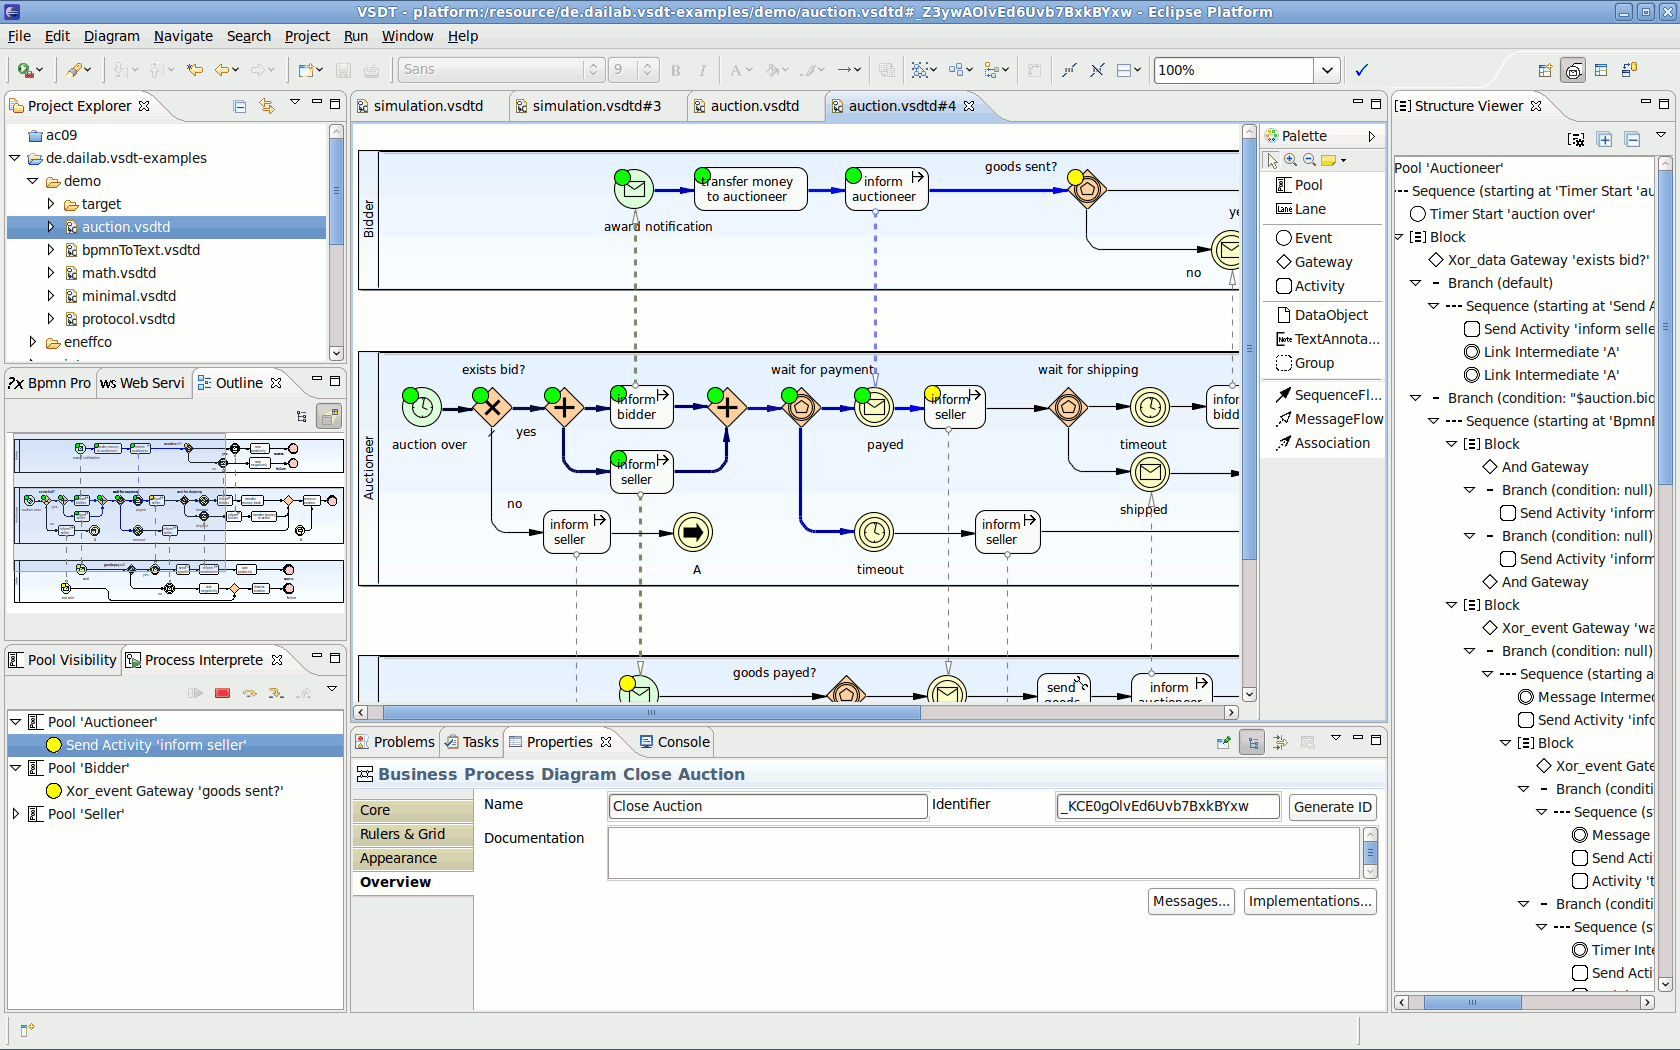
\includegraphics[height=.4\textheight]{figures/vsdt_1-3-0.png}
	\caption[The Visual Service Design Tool]{The Visual Service Design Tool.
	Clockwise: Graphical Editor (with running Simulation), Structure Viewer,
	Property View, Process Interpreter View, Visual Outline, Navigator.}
	\label{fig:screen}
\end{figure}


\subsection{The Metamodel}

% Ueber die BPMN Spezifikation und wie sie umgesetzt wurde
The BPMN specification~\cite{omg2009bpmn} describes in detail how the several
nodes and connections constituting a BPMN diagram have to look, in which context
they may be used and what attributes they have to provide.  However, it does
neither give a formal definition of the syntax to be used for the meta-model, nor
an interchange format, e.g. using an XML Schema Definition (XSD).  Thus the
editor's meta-model had to be derived from the informal descriptions in the
specification.  As it was our main concern to keep as close to the specification
as possible, almost every attribute and each constraint given in the specification
have been incorporated into the meta-model, allowing the creation of any legal
business process diagram.  Still, some attributes have not been adopted in the
meta-model: For instance the possibility to model nested or even crossing Lanes
has been dropped, as it turned out that this feature seems to be virtually never
used in practical business process design.


\subsection{The BPMN Editor}

% Basis: Eclipse GMF -> Viele gute Features frei Haus
Like many others, the VSDT editor has been created using the \emph{Eclipse Graphical
Modelling Framework (GMF)}, automatically equipping the editor with numerous
features, such as support for the Eclipse properties, outline and problem view
and unlimited undo and redo, just to name a few.  Being embedded in the Eclipse
workbench, the editor is easy to use while at the same time providing a powerful
tool for professional business architects and service developers.

% Erweiterungen: Property Sheets, Dialoge, Validierung, etc.
While GMF provides a solid basis for the editor, several customizations have been
made to the code, further improving the editor's overall usability and supporting
the creation of new business processes.  For example, the generated property
tables have been supplemented with custom-made sheets, in which the several
attributes are more clearly arranged.  For managing the non-visual elements given
in the BPMN specification, such as Properties, Messages and Assignments, a number
of clear and uniform dialogs were created.  The various constraints given in the
specification were translated to several audit constraints used to validate a
given business process diagram.

% Nachteil der Erweiterbarkeit/ BPEL-unabhaengigkeit: keine BPEL-Untertuetzung im Editor
As already mentioned, the VSDT was designed to be a pure BPMN editor and independent
of BPEL, so the business process diagrams can be transformed to other languages,
too, given the respective export plug-ins.  Of course, the downside of this approach
is that the editor lacks built-in support for BPEL, e.g.\ the editor itself does
not validate an expression given in the diagram to conform to the BPEL syntax.
However, it is possible to supplement the editor with additional plug-ins, which
can contribute e.g.\ to the property sheets or provide whole new views with
language-specific functionality.

% Rich Service Directory
One example of how the VSDT can be extended with features specific to a certain
target language --- in this case: BPEL --- is the Web Service View, which can bee
seen in Figure~\ref{fig:screen}, too.  Using the Web Service View, existing Web
services can be inspected and imported into the diagram.  In the process, an
Implementation object is created for the Web service as well as a set of Message
objects, matching the service's input parameters and result.  Optionally, also a
new Pool will be created for the service, which can be connected to the currently
selected Activity via a pair of Message Flows.  Further, the Implementation and
the Message objects will be associated to the Activity and its type will be set
to \textsc{service}.  Thus, the orchestration of existing Web services in a BPEL
process can be simplified greatly.  Similar features can be created for other
target languages, too.

% Export Wizards
Once the business process diagram is completed, it can be validated and exported
to an executable language, such as BPEL or the JIAC agent framework.  As the VSDT
is intended to provide export features to arbitrary target languages, and to
support developers in the creation of these features, we have created an elaborate
export framework.  For each of these features, being realized as additional
Eclipse plug-ins, an individual wizard can be made available in the Export menu.

For more information regarding the Visual Service Design Tool, please refer
to~\cite{kuester2008towards}.


%%%%%%%%%%%%%%%%%%%%%%%%%%%%%%%%%%%%%%%%%%%%%%%%%%%%%%%%%%%%%%%%%%%%%%%%%%%%%%%%
%%  Features                                                                  %%
%%%%%%%%%%%%%%%%%%%%%%%%%%%%%%%%%%%%%%%%%%%%%%%%%%%%%%%%%%%%%%%%%%%%%%%%%%%%%%%%

\section{Features}

% Stand: Version 1.4.0

In the following, some of the features of the VSDT are listed.  For more information
on selected features, please refer to Section~\ref{sec:user_features}.

\begin{itemize}
	\item export to (and import from) executable BPEL and JIAC Code and STP-BPMN
	\item translation of Expressions to the language used in the target framework
	\item process simulation and interpretation
	\item BPMN-to-text generation
	\item combination of BPMN-diagrams with Use-case-like 'higher view'
	\item pattern-based modeling, insertion of pattens on existing edges
	\item quick assembly of process diagrams using keyboard-shortcuts
	\item quick assignment of service parameters
	\item dynamic filtering of displayed pools
	\item variables-view and similar tools for the management of non-visual elements
	\item verification of process structure at design time
	\item automated, structure-based layout of BPMN diagrams
	\item one-click deployment of JIAC agent services generated from BPMN diagrams on a JIAC runtime
\end{itemize}



%	\part{User's Guide}
	\chapter{Setup}
\label{sec:user_setup}

In the following the installation process for the VSDT will be explained.  As the
VSDT is a plugin to the Eclipse IDE, the installation process is subdivided in
several steps:
\begin{enumerate}
	\item Install Eclipse
	\item Install Dependencies
	\item Install VSDT
\end{enumerate}

\emph{Note} that for running the VSDT Version 5 of the Java environment is required.

\emph{Note} that the versions of the dependencies may vary depending on the
version of the VSDT.  The following applies to version \version of the VSDT.


%%%%%%%%%%%%%%%%%%%%%%%%%%%%%%%%%%%%%%%%%%%%%%%%%%%%%%%%%%%%%%%%%%%%%%%%%%%%%%%%

\section{Installing Eclipse}
\label{sec:user_setup_eclipse}

For using the Visual Service Design Tool you need the Eclipse IDE which can be
downloaded from \url{http://www.eclipse.org} for different operating systems.

The VSDT \version\ works with Eclipse 3.5 ``Galileo''.\footnote{For Eclipse 3.4
you can still use the VSDT up to version 1.2.2.}


%%%%%%%%%%%%%%%%%%%%%%%%%%%%%%%%%%%%%%%%%%%%%%%%%%%%%%%%%%%%%%%%%%%%%%%%%%%%%%%%

\section{Installing Dependencies}
\label{sec:user_setup_dep}

The VSDT depends on a number of other plugins which again will have some
dependencies on its own.  It is recommended to use the Eclipse Update feature, as
in that case all the dependencies and the dependencies of the dependencies will
automatically be installed, too.  The dependencies are:

\begin{itemize}
	\item Graphical Modeling Framework SDK (group ``Modeling'')\footnote{The VSDT
	\version\ was created with GMF 2.1 and has been adapted to work with GMF 2.2.}
	
	\item XText SDK (group ``Modeling'')
\end{itemize}

For installing the plugins, make sure you are allowed to write in the Eclipse
program folder, especially when running Linux you should start that instance of
Eclipse with \texttt{sudo}.  In Eclipse, select \emph{Help} from the menu, then
\emph{Install New Software...}.  Select the \emph{Galileo} repository from the
drop-down menu and select the Dependencies from the list below.  Now click on
\emph{Next} to automatically check calculate further dependencies and continue
through the installation process.  After that you might have to restart Eclipse.
If the installation was successful the new features should appear in the
\emph{Installed Software} tab of the same dialog.

Theoretically, Eclipse can resolve the dependencies on its own, so it should be
enough to select the VSDT itself.  Still, we recommend to install the dependencies
manually.


%%%%%%%%%%%%%%%%%%%%%%%%%%%%%%%%%%%%%%%%%%%%%%%%%%%%%%%%%%%%%%%%%%%%%%%%%%%%%%%%

\section{Installing the VSDT}
\label{sec:user_setup_vsdt}

Once Eclipse and GMF are set up you can install VSDT.  The Visual Service Design
Tool consists of the following features:

\begin{itemize}
	\item \emph{VSDT: Visual Service Design Tool} This is the core component of
	the VSDT, the visual BPMN editor, along with a number of useful extensions
	and the basic transformation framework.

%	\item \emph{VSDT: RSD Integration} This feature contributes an additional
%	view to the BPMN editor, making the reuse of existing Web services easier.

%	\item \emph{VSDT: Transformation Base} This is an enabling feature for the
%	several export features, providing the common functionality and look and
%	feel for the transformations.

	\item \emph{VSDT: BPMN - BPEL Transformation} This feature provides the export
	to executable BPEL code.

	\item \emph{VSDT: BPMN - JIAC V Transformation} This feature provides the
	export to JIAC V multiagent-systems.  Additional Dependency: \emph{Agent World
	Editor}

	\item \emph{VSDT: BPMN - STP-BPMN Transformation} This feature provides
	exchange with the popular Eclipse STP BPMN editor.  Additional Dependency:
	\emph{BPMN Project Feature} (

	\item \emph{VSDT: BPMN - \dots Transformation} Further export and import
	features will be released over time, providing transformations to other
	languages, such as JIAC agents.
\end{itemize}

The VSDT can be obtained from the following sites:
\begin{center}
	\downloadsites
\end{center}

Download the VSDT as an archived update site and add the site in the \emph{Install
New software} dialog (see last section), using the \emph{Add...} button.


	\chapter{The Perspective}
\label{sec:user_perspective}

This section will briefly introduce those parts of the Eclipse GUI that are
relevant for the work with the Visual Service Design Tool.  These views are
aggregated in the Easy Service Creation perspective, which an be selected via the
Menu \emph{Window $\rightarrow$ Perspective}.  Figure~\ref{fig:screen}
(page~\pageref{fig:screen}) is showing a screenshot of the Visual Service Design
Tool featuring most of the relevant views.  In the following each of the views
will be introduced briefly.


%%%%%%%%%%%%%%%%%%%%%%%%%%%%%%%%%%%%%%%%%%%%%%%%%%%%%%%%%%%%%%%%%%%%%%%%%%%%%%%%

\section{VSDT Editor Views}
\label{sec:user_perspective_editor}

The editor window is shown automatically when opening a file in the Navigator
view.  Depending on the PlugIns currently installed this can be a plain text
editor, a browser, an elaborate code editor or some sort of graphical editor.
For the Visual Service Design Tool there are two editors available: A visual
editor showing the BPMN graph and a tree editor reflecting the internal structure.

\paragraph*{The Graphical Editors}
These are the primary editors when working with the VSDT (see
Figure~\ref{fig:screen_meta}):

\begin{figure}
	\centering
	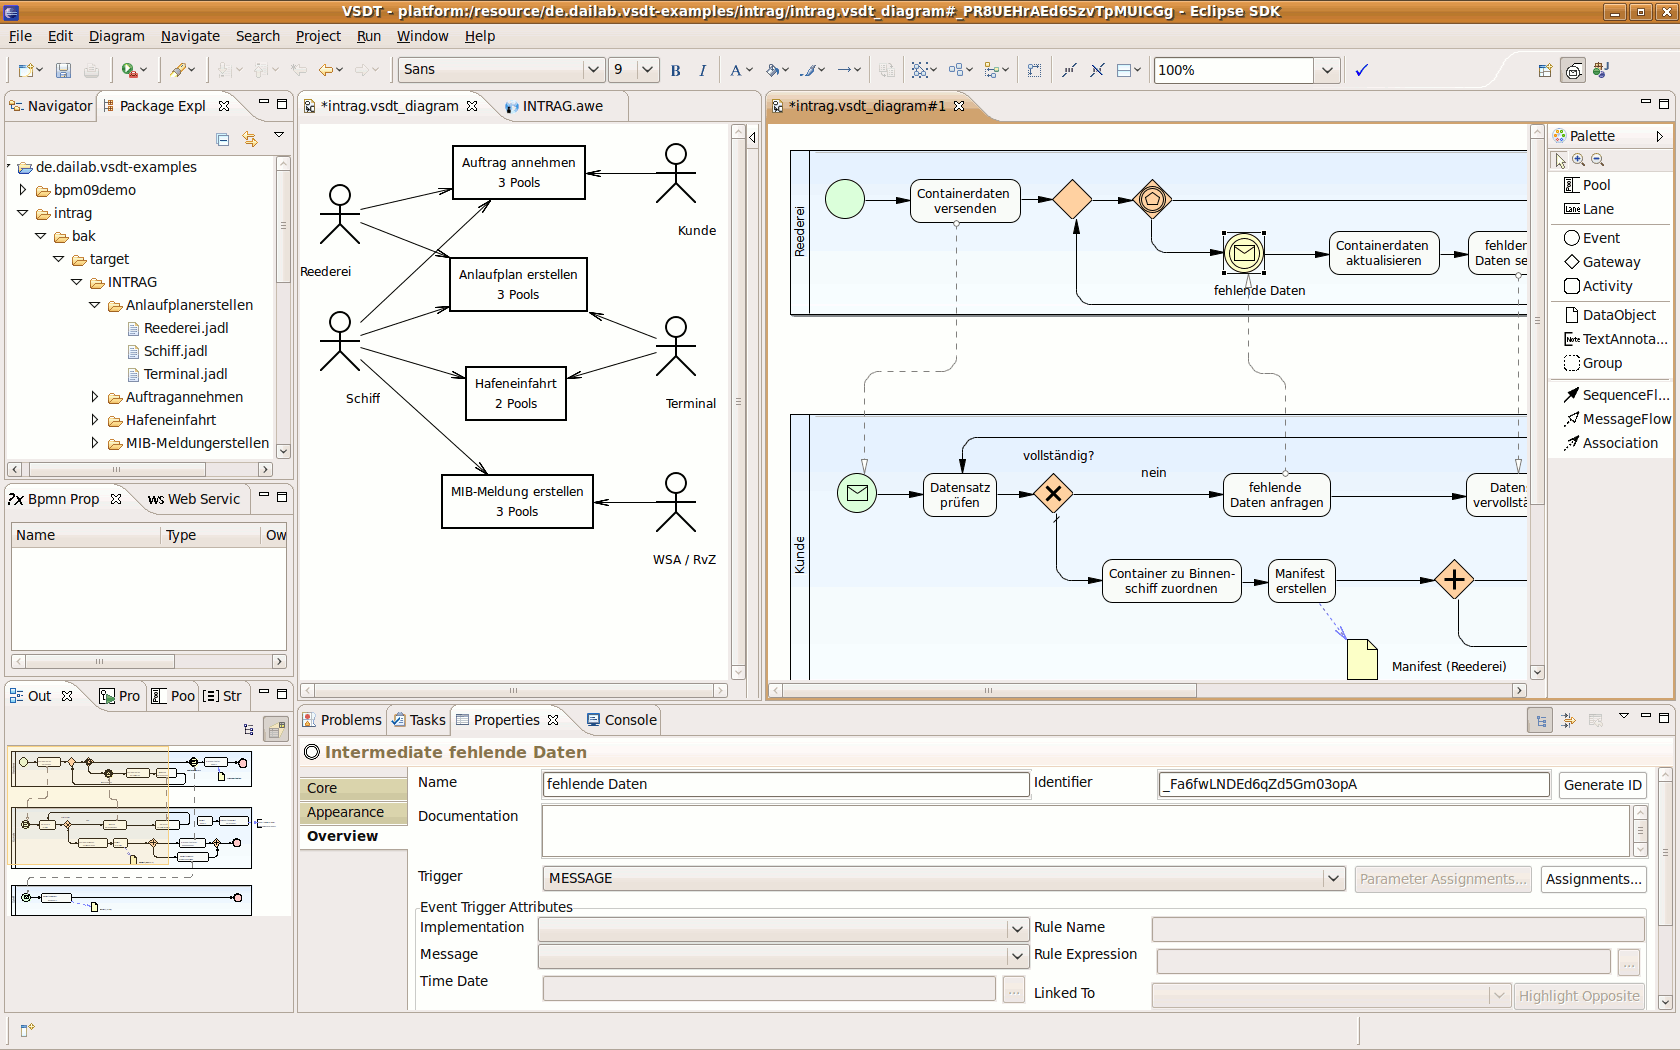
\includegraphics[height=.4\textheight]{figures/vsdt_1-3-0_uc.png}
	\caption{Business Process System and BPMN editor shown side-by-side.}
	\label{fig:screen_meta}
\end{figure}

\begin{itemize}
	\item The \emph{Business Process System} editor is opened when the diagram
	file is clicked.  It is used for organizing the several interdependent Business
	Processes which make up the system as a whole, as well as the Participants
	involved in these Processes.
	
	\item The \emph{Business Process Diagram} editor is opened when double-clicking
	one of the Business Process Diagram nodes in the Business Process System
	editor.  This editor is the actual BPMN editor used for modelling the
	individual Business Processes.
\end{itemize}

Both editors feature a palette with the nodes and connections.  For placing a
node on the canvas or inside a compartment of another node (e.g. a Pool or a Sub
Process) click the icon in the palette and then click again on the canvas.  For
drawing connections, click on the first node, draw the connection to the second
node and release the mouse button.  Note that nodes and connections can not be
drawn arbitrarily, but have to follow the BPMN syntax, e.g. a Task can only be
drawn inside a Pool and a Sequence Flow can only connect Flow Object within the
same Pool.

\paragraph*{The Tree Editor}
The tree editor can be useful for managing and editing those parts of the Business
Process Diagram that do not have a graphical representation.\footnote{Although in
general it is not necessary to use the tree editor, as the graphical editor
provides means for editing non-graphical elements, too.} Note that the tree editor
is more powerful than the graphical editor, and the diagram might be invalidated
when doing certain operations in the tree editor.  Especially, the tree editor
should \emph{not} be used for creating any elements that \emph{do} have a graphical
representation in the diagram, as this representation will not be created along
with the element.

\paragraph*{The Text Editor}
Both the diagram and the model file can be opened with any text editor and edited
as XML.  While this can be helpful for adapting existing models to changes in the
metamodel of a newer version of the VSDT, you should in general avoid editing the
files XML sources, as this can render them unreadable for the other editors.


%%%%%%%%%%%%%%%%%%%%%%%%%%%%%%%%%%%%%%%%%%%%%%%%%%%%%%%%%%%%%%%%%%%%%%%%%%%%%%%%

\section{General-purpose Eclipse Views}
\label{sec:user_perspective_general}

In the following those standard views of the Eclipse IDE will be introduced, that
are relevant for the work with the VSDT.

\paragraph*{The Project Explorer}
Here the user can manage his projects and create and delete files.  Note that
Eclipse provides different similar views for managing files, e.g. the Project
Explorer, Navigator, or the Package Explorer, each providing slightly different
features.

\paragraph*{The Properties View}
Although some attributes, like an element's name, can be edited in the graphical
editor view as well, for most other attributes the properties view will be needed,
where all the attributes relevant to the user can be inspected and edited.  Of
course, each change done in the properties view can be undone and redone and the
editor will be immediately updated.  There are two tabs available in the properties
view: The \emph{Core} tab provides a table showing the attributes in categories
and in alphabetic order.  The \emph{Overview} tab provides a clearer look, grouping
the attributes and arranging them by relevance in two columns.  Additionally, the
Outline tab features a number of buttons, providing access to additional dialogs
for managing e.g.\ an Activity's Properties and Assignments.

\paragraph*{The Outline}
This view provides a short outline of the current editor's content.  In case of
a graphical editor, like the VSDT, this can be a miniature view of the entire
diagram, and in case of a tree editor an additional tree view for easier navigation.

\paragraph*{The Problem View}
This view lists all the problems that have been found in the model, subdivided in
errors and warnings.  By double-clicking one of the items the editor will focus
on the element the problem occurred on (for refreshing the errors shown in the
Problem View, select \emph{Diagram | Validate} from the menu).

\paragraph*{The Error Log}
Other than the Problem View, the Error Log will log problems with the editor
itself.  So if you encounter strange behaviour or in case the editor should crash
you can check here for the reason and send in an error report.


%%%%%%%%%%%%%%%%%%%%%%%%%%%%%%%%%%%%%%%%%%%%%%%%%%%%%%%%%%%%%%%%%%%%%%%%%%%%%%%%

\section{Additional Views for the VSDT}
\label{sec:user_perspective_custom}

The following are views that have been crafted especially for the VSDT.

\paragraph*{The BPMN-Properties View}
\label{sec:user_perspective_propView}

The BPMN-Properties View (see Figure~\ref{fig:customViews}, to the left) provides
an easy way to inspect the Properties in the scope of the currently selected
element in the active editor, i.e. the Properties that can be used in an Assignment
owned by that element.  The property scope of a BPMN element comprises the
Properties of (a) that element itself, e.g. an Activity, (b) Messages going in
and out of that element, e.g. the in- and output parameters of a Web service call,
and (c) the (transitive) parents of that element, e.g. (Sub-) Processes.

\begin{figure}[t]
	\centering
	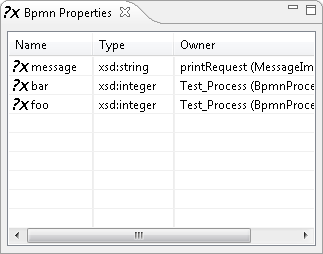
\includegraphics[width=.3\textwidth]{figures/features/propView.png}
	\hspace{.5cm}
	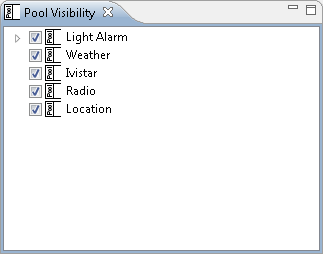
\includegraphics[width=.3\textwidth]{figures/features/poolView.png}
	\hspace{.5cm}
	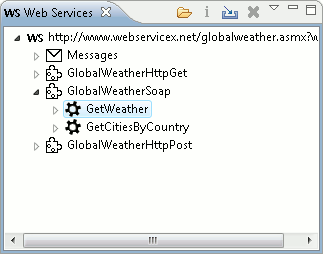
\includegraphics[width=.3\textwidth]{figures/features/wsView.png}
	\caption{The BPMN Properties View, Pool Visibility View, and Web Service View.}
	\label{fig:customViews}
\end{figure}

The Properties are displayed in three columns, showing the name and the type of
the Property and the name and the element type of the Property's parent element.
The properties an be sorted by clicking on the column heads.  By double-clicking
on a Property, an Organize Properties Dialog will be opened for the Property's
parent element.

\paragraph*{The Pool Visibility View}

In the Pool Visibility View, which is seen in the centre of Figure~\ref{fig:customViews},
all the Pools in the diagram are displayed.  If the check box in front of an entry
is unchecked, the corresponding Pool and all incoming and outgoing connections,
e.g.\ Message Flows, will be hidden.  This feature can be of some use in diagrams
holding many Pools: When modelling three or more interconnected Pools, Message
Flows going from the first to the third Pool might cross the second Pool, which
can be confusing when editing that Pool.  In this case, the first or the third
Pool may be hidden, so the Message Flows (which are then hidden, too) do not
longer obstruct the view on the second Pool.  In the same way the Pools and
Message Flows can be shown again by checking the corresponding check box.  Note
that these settings are not persisted, so when closing and re-opening a diagram
all Pools will be visible again.
%	Further, the Pool entries can be expanded, showing an outline of the elements
%	within.  However, this feature, which might some day supplement the Outline View,
%	is still at an early stage.

%	\paragraph*{The RSD View}
%	The RSD view can be used to inspect and import Web services into the process
%	diagram.  Using the RSD View not a single Web service is inspected, but the
%	content of a \emph{Rich Service Directory}, a special kind of Web service
%	repository also capable of advertising services and operations from other sources,
%	e.g.  UPnP devices or JIAC TNG actions.  The several operations of each Web
%	service registered at the Rich Service Directory are displayed in a list from
%	which they can be selected, inspected, and imported into the diagram.  When
%	importing Web services, the corresponding Web service descriptions and input and
%	output messages will be created automatically.  However, the RSD implementation
%	is still at an early stage, and thus by now the use of the RSD View is limited.

\paragraph*{The Web Service View}
%	Similar to the RSD View, this view can be used to inspect and import Web service
%	descriptions into the active BPMN diagram.  However, other than using the RSD
%	view, the Web Service view does not need the RSD but will directly connect to a
%	given Web service URL.
The Web Service View (see Figure~\ref{fig:customViews}, to the right) provides
access to Web Services, which can be inspected and imported into the currently
opened diagram.  Web Services can be added to the list by clicking the Open button
and entering the exact URL of the WSDL definitions file.  The Web Service is
displayed as a tree, including the various Messages and their types, nad the Port
Types, their Operations, and their In- and Output Messages.  By clicking the Info
button, the complete WSDL definition is shown in plain XML.  Most importantly,
Messages and Operations can be imported from the Web service description into the
Business Process Diagrams, so they can be reused in a Web service invocation.

\paragraph*{The Interpreter View}
\label{sec:user_perspective_simView}
BPMN diagrams created with the VSDT can be simulated and interpreted using the
built-in process interpreter (see Figure~\ref{fig:customViews2} and
Section~\ref{sec:user_features_sim}).  For starting a simulation, first switch to
the BPMN diagram you want to simulate.  Open the Process Interpreter View and
click the \emph{Start} button.  For each Pool in the diagram, the view will show
those Activities that are currently \textsc{active} or \textsc{ready}.  For
advancing a step in the simulation, expand a Pool and double-click one of the
listed elements, that is the Flow Objects currently being ready, e.g.\ Start
Events.  For more control, you can also select one of \emph{Step Over}, \emph{Step
Into} or \emph{Step Out}.  Hit the Stop button for ending the simulation and
removing the markers from the diagram editor view.

\paragraph*{The Structure View}
\label{sec:user_perspective_strucView}
This view allows to apply the Structure Mapping (see~\ref{sec:user_trafo_intro})
at modelling time, displaying the results in a tree.  By clicking on an element,
the corresponding node in the diagram is highlighted.  Further, the user is
notified if there seem to be structural conflicts in the process, which is
determined from the number of left-over Sequence Flows.  This view should prove
highly useful for validating the structure of processes prior to transformation
to executable code (see Figure~\ref{fig:customViews2}).

\begin{figure}[t]
	\centering
	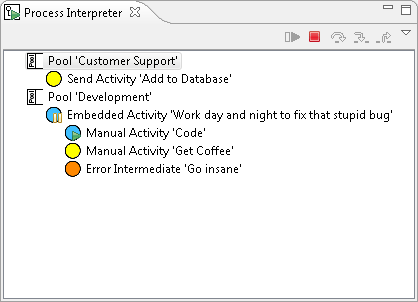
\includegraphics[width=.4\textwidth]{figures/features/interpreterView.png}
	\hspace{.5cm}
	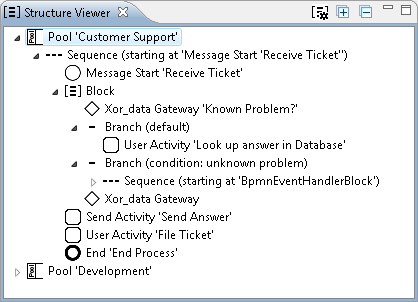
\includegraphics[width=.4\textwidth]{figures/features/structureView.png}
	\caption{The Interpreter View and Structure View.}
	\label{fig:customViews2}
\end{figure}


	\chapter{Basic Tutorial}
\label{sec:user_tut}

In this chapter the user will be guided through the creation of a simple Business Process Diagram,
from creating the diagram file to validation and code generation.


\section{Creating a new Business Process Diagram}
\label{sec:user_tut_new}

These are the basic steps for creating your first Business Process Diagram:

\begin{enumerate}
	
	\item Start Eclipse and select a location for the workspace. This is where all the projects --
	BPMN and others -- will be stored. When starting Eclipse for the first time, a welcome screen
	will be shown. Read something about the features of Eclipse, if you want, then exit the screen.
	
	\item Change to the \emph{VSDT} Perspective.
	
	\item Select \emph{ New $\rightarrow$ Project $\rightarrow$ General $\rightarrow$ Project } in
	the menu bar. Open the Navigator View to see the newly created Project.
	
	\item On the project, select \emph{New $\rightarrow$ VSDT Meta Diagram} and enter a name for the
	file. On the last page of the wizard some of the global settings for the Business Process
	Diagram, such as the Title, Description and Author name, can be set. A file with the extension
	'vsdtd' is created, holding both the semantic model and the notational model (i.e. the layout
	information).
%	Two files will be created. The first file, \verb|$NAME.vsdt_diagram| is holding the layout
%	information for the diagram, while the other one, \verb|$NAME.vsdt|, is for the pure model data.
	
	\emph{Note} that the files are stored in XML format and can be edited with a text editor, too.
	However, you should do so only to fix a broken file.
%	The diagram file can be recreated from the model file by right clicking it and choosing to
%	initialize the diagram file.
	
	\item By now, the diagram should have opened automatically; otherwise open it manually by
	double-clicking it. It will be opened with the graphical editor. 
%	For now, ignore the model file.

\end{enumerate}


\section{Setting up Participants and Business Processes}
\label{sec:user_tut_meta}

With the VSDT, not only individual Business Process Diagrams, but sets of Business Process Diagrams
belonging to the same scenario -- here referred to as Business Process Systems -- can be modelled.
For this, the modelling starts with defining the several Participants and the Business Processes
they participate in.

\begin{enumerate}

	\item Select a \textbf{Participant} from the palette and click on the canvas. A stick-figure
	will appear. Repeat for each Participant relevant for the Business Process System. These can be
	companies, roles, computer systems or individual persons.
	
	\item Now select \textbf{Business Process Diagram} from the palette and draw it on the canvas.
	These represent the individual processes (quite similar to 'Use cases').
	
	\item Now select the connection form the palette and connect the Participants with the Business
	Processes.
	
	\item Finally, perform a double-click on one of the Business Process Diagram nodes, which will
	open it in a new diagram editor.
	
\end{enumerate}


\section{Modelling a basic Business Process}
\label{sec:user_tut_basic}

Next, we will formulate a simple business process. Here, we will focus on the visual elements of
BPMN.

\begin{enumerate}

	\item To get started, perform a right-click on the canvas and select \emph{Initialize
	$\rightarrow$ Initialize Pools} and hit \emph{OK} to confirm the dialog. For each Participant
	associated with the Business Process a Pool will be created.
	
	\item Alternatively, select \textbf{Pool} from the top of the palette and move the mouse to the
	canvas. Push the mouse button and drag it to the lower right to create a large Pool. Enter a
	name for the Pool and select one of the Participants associated with the Business Process using
	the Properties view.
	
	\item Along with the Pool also a Lane will be created. To create more Lanes, select the
	\textbf{Lane} element from the palette and click on the Pool's label (as existing Lanes will
	fill the Pool's compartment completely). Note that the Lanes can not be moved manually.
	According to the BPMN specification the first Lane will be invisible (faded out in the editor).
	
	\item Let's create some \textbf{Flow Objects} inside of the Lane. Select one of the Flow Object
	from the palette, i.e. Events, Activities and Gateways, and click inside of the Lane. In case
	you selected the Event, a small menu will appear, asking whether to create a Start, End, or
	Intermediate Event; otherwise the element will be created right away.
		
	\item Select the \textbf{Sequence Flow} icon from the palette and connect the several Flow
	Objects by pressing the mouse button on the source and dragging it to the target. When
	connecting the Activity be sure to aim for the label. If you hit the Activity's compartment you
	can not create a connection. You can change the routing style from the toolbar or add more
	bendpoints to a connection by dragging it.
	
	\item Use the Property Sheets to alter the Elements' name, description, type, and type-specific
	attributes. Select the element, e.g.\ an event, and open Eclipse's Property View. Select the
	Overview sheet from the tabs to the left to find a clearly arranged form holding the various
	attributes. If you want to set only the type of a Flow Object, e.g. for making an Event a
	\emph{Message} Event, you can also use the element's context menu and select \emph{Edit...
	$\rightarrow$ Set Type}, or use the keyboard shortcut \texttt{Ctrl+T}.

	\item Now select the \textbf{Message Flow} icon from the palette. Select an Activity or an End
	Event as source and draw the Message Flow to an element in a different Pool, or to some point
	beneath the Pool and select to create a new Pool element there.
		
	\item Finally, we will associate an Activity with a \textbf{Data Object} (however, this will not
	affect the generated BPEL code). Select the Data Object from the palette and create it on the
	canvas. Select the Association connection from the palette and connect the Data Object to the
	Activity. Select \emph{BPMN $\rightarrow$ Initialize Input/Output Set} from the Activity's
	context menu, depending on the associations direction. Notice the new Input Element in the
	Activity's property sheet. This Input Set references all the Activity's incoming/outgoing Data
	Objects.
	
\end{enumerate}


\section{In-depth Modelling}
\label{sec:user_tut_ws}

Now that we created the diagram visuals, this section deals with the equally important underlying,
non-visual parts of BPMN, such as properties, assignments, conditions, and service invocations.

%\emph{Note:} In case of the export to BPEL this will map to a Web service call, but can map to
%similar concepts, too, depending on the target language.

\begin{enumerate}

%	\item Select the Pool, open its Overview property sheet and select a \textbf{Participant}. In
%	case no Participants are defined yet -- which is likely -- hit the \emph{new Participant} button
%	in the Pool's property sheet. Participants are the ``owners'' of the Pools. Since one
%	Participant can own several Pools, a Participant is not created automatically for each Pool.
	
	\item Right-click the Message Flow or open its property sheet and select \emph{Initialize
	Message}. Note that by doing so the End Event's type changes to \texttt{Message}. A new
	(non-visual) Message object has been created and associated with the Message Flow, and its
	source and target, if possible.
	
	\item To define a (Web-) service invocation, select the \emph{Organize Implementations} and
	\emph{Organize Messages} buttons from the Business Process Diagram's property sheet. Select the
	newly created Messages and Implementations (services) from the list and set the values according
	to the service to invoke. Alternatively, Web services can also be imported using the Web Service
	View, which is much more comfortable and will be explained in depth later.

	\item Next, we will define the process data, i.e. Properties associated to the Pool's Process.
	Open the Pool's overview property sheet and click \emph{Organize Process Properties} or select
	the respective item from the Pool's context menu. Create some properties using the buttons in
	the shown dialog and edit the values of the selected Property using the text fields in the lower
	part of the dialog. Besides the top-level process, Tasks and Subprocesses can hold Properties,
	too, which are available only for that activity or its child activities, if any.
	
	\item To assign a value to a Property, you have to create an Assignment. Open the properly sheet
	of some element in the process and click the Assignments button. Create a new Assignment, select
	the Property and enter an Expression. Click the button with the dots (\dots) on it to open
	another dialog helping you to enter and validate an expression using the VSDT Expression
	Language VXL (see Appendix~\ref{sec:vxl}).
	
	\item Now that the Properties are declared and assigned a value, they can be used e.g.\ in
	condition expressions. Select a Sequence Flow coming from a Gateway (a point where the flow of
	control branches), set the Condition Type to \emph{Expression} and enter the Condition
	Expression. Again, use the button with the three dots(\dots) to validate the Expression.
	
	\item Just like Processes and Activities, Messages can have Properties. Again, the dialog can be
	accessed via the property sheet or the context menu. Add some properties to the newly created
	Message(s), being the input and output parameters of the respective Web service.
	
	\item To pass the parameter values to the Message, create one or more Assignments on the Flow
	Object the Message is going in or out of. There are two ways for doing this:
	\begin{itemize}
		\item The easiest way is to use the \emph{Parameter Assignment Dialog}. Select the Activity
		or Event sending or receiving the Message(s) and hit the respective button in its property
		sheet. The dialog will show all of the messages' input and output Properties and offer
		drop-down menus for selecting another Property or entering an individual Expression to be
		assigned to these parameters.
		\item For more control over the parameter assignments, you can also open the \emph{Organize
		Assignment Dialog} via the Flow Object's property sheet or context menu and manually create
		the individual Assignments. Select a Property to assign the value to, e.g. one of the input
		parameters of the Web service's input message, and enter a from expression.
	\end{itemize}
	 To refer to a Property in the expression, just type in the Property's name with a leading
	 \verb|$|, e.g. \verb|$foo + 1|. Note the assign time value: if this is set to before, the
	 assignment will be made before the Activity is executed, i.e. the Web service is invoked,
	 otherwise the assignment will be made afterwards. Thus this value should be set to
	 \emph{before}, when passing values from the process to a Web service's input parameter, and to
	 \emph{after}, when passing values from the Web service's output parameter back to the process.
\end{enumerate}


\section{Validation and Simulation}
\label{sec:user_tut_validation}

When your process is done -- or seems to be done -- you should validate it. There are several means
for validation in the VSDT: First, you can validate the process diagram against the constraints
given in the BPMN specification; second, you can check the structure of the process, which is
important for most transformations to executable code; and third, you can run a simulation, testing
the several Expressions, Conditions, and Assignments.

\begin{enumerate}

	\item To validate the diagram against the constraints from the BPMN specification, select
	\emph{Diagram $\rightarrow$ Validate} from the menu, or by clicking the checkmark symbol in the
	tool bar. You might notice some error or warning marks in your diagram or entries in the problem
	view. You should fix these problems before exporting the diagram to executable code and validate
	the diagram again.
	
	\item For checking the structure of the process, open the Structure View (see
	Section~\ref{sec:user_perspective_strucView}) and click the \emph{Structurize} button. This will
	trigger the same Structure Mapping used in the actual transformations and display the result,
	i.e. a structured form of the process, featuring elements such as sequences and blocks. While
	the structured model might be a bit cumbersome to read, it gives evidence of the structure that
	will be recognized from the process, and if this is not the structure you intended you should
	consider restructuring the process. Unfortunately, most executable languages are much more
	restrictive than process notations such as BPMN, so this check is necessary.
	
	\item For a more in-depth validation of the process you may consider running a simulation.
	Currently there are two types of simulations implemented: a manual simulation and an
	interpreting simulation (see Section~\ref{sec:user_features_sim}).
	\begin{itemize}
		\item Use the manual simulation to get a feel of how the process behaves when taking a
		certain path, and to identify possible deadlock situations
		\item When using the VSDT Expression Language (VXL, see
		Section~\ref{sec:user_features_exp}), the interpreting simulation will help you validating
		the several condition and assignment expressions used throughout the process.
	\end{itemize}

\end{enumerate}


\section{Code Generation}
\label{sec:user_tut_export}
	
Once all three validations are successful, the diagram can be translated to executable code. Of
course, there might still be semantic errors in the process the validation can not uncover, so you
should think about thoroughly testing the resulting program code before deploying it to productive
use.
	
\begin{enumerate}

	\item Once the diagram shows no more errors, it can be exported to executable code. Select
	\emph{Export...} from the file menu or from the model file's context menu. Select the desired
	target language from the \emph{BPMN Export} group and proceed through the dialog. Select the
	model file(s) to be exported, adjust the target directory or the other options, if necessary,
	and hit the \emph{Finish} button.
	
	\item The export might take some seconds. If the model is sound, the output files will be
	created in a new directory in the specified target directory, named after the Business Process
	Diagram. By default, also a log file will be created along with the model files in the directory
	\emph{exportLogs} in the specified target directory.
	
	\item If the process has been modelled accurately, the resulting program can be readily
	executable. Still it is recommended to check the result with a native editor for the respective
	language, to be sure the files are free from defects.

\end{enumerate}

	\chapter{Selected Features}
\label{sec:user_features}

This chapter will give further insight on how to use some of the features of the Visual Service
Design Tool.


\section{GMF Modelling Assistance}
\label{sec:user_features_assistance}

The Eclipse Graphical Modelling framework the VSDT is based upon comes with a number of valuable
modelling assistance features (if not desired, modeling assistance can be turned off in the
preferences). In the following some of these will be briefly introduced. Figure~\ref{fig:modAss} is
showing the modelling assistance in use.

\begin{itemize}
	\item When resting the mouse on top of a compartment, a small palette will show up, showing the
	elements that can be placed in this compartment. Thus one does not have to go all the way back
	to the palette for creating a new node.
	\item When resting the mouse on top of a node, small arrows going in and out of the node will
	appear. By dragging these arrows new connections can be drawn.\footnote{Depending on the
	location, different connections will be offered: In the top and bottom region of a node incoming
	and outgoing Message Flows, in the left half incoming Sequence Flows and Associations, and in
	the right half outgoing Sequence Flows and Associations respectively.}
	\item When a connection is drawn and the mouse button is released over the canvas or another
	compartment, a node can be created in that place along with the connection.
	\item In case multiple node- or connection-types can be created using a given tool in a given
	context, the user will be prompted to select one.
\end{itemize}

\begin{figure}[ht]
	\centering
	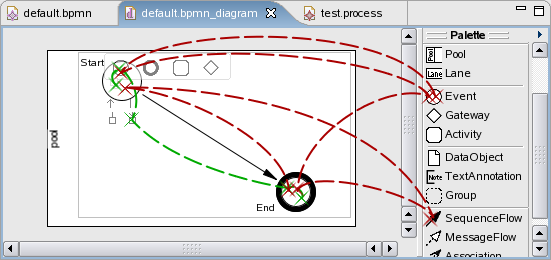
\includegraphics[width=.5\textwidth]{figures/features/modellingAssistant.png}
	\caption{Mouse movement with and without the use of the Modelling Assistant.}
	\label{fig:modAss}
\end{figure}


\section{Managing Non-Visual Elements}
\label{sec:user_features_nonvis}

For each of the non-visual elements --- Properties, Assignments, Messages, and Implementations--- a
management dialog has been written. The dialogs follow a clear and recognizable layout, showing the
elements as-is in a list along with a number of buttons for inserting, removing and sorting of the
elements and text fields for editing the attributes of the currently selected item (see
Figure~\ref{fig:dialog}).

\begin{figure}[ht]
	\centering
	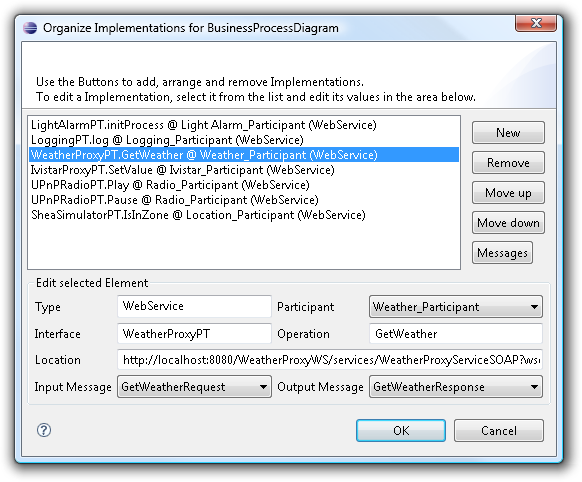
\includegraphics[width=.5\textwidth]{figures/features/dialog.png}
	\caption{A Supporting Type Organization Dialog.}
	\label{fig:dialog}
\end{figure}

The various dialogs can be accessed in the following ways:
\begin{itemize}
	\item The Organize Properties Dialog can be accessed via the context menu and property sheet of
	Pools, Activities and Message Flows, and by double-clicking an element in the BPMN-Properties
	View or a Message Flow.\footnote{In the case of Message Flows, the Properties of the underlying
	Message, if any, will be edited, and in the case of Pools, the Properties of the Pool's
	Process.}
	\item The Organize Assignments Dialog can be accessed via the context menu and property sheet of
	Pools and Flow Objects, and by double-clicking Flow Objects.
	\item The Organize Messages Dialog can be accessed via the context menu and property sheet of
	the Business Process Diagram and the property sheet of Message Flows.
	\item The Organize Implementations Dialog can be accessed via the context menu and property
	sheet of the Business Process Diagram.
%	\item The Organize Participants Dialog can be accessed via the context menu and property sheet
%	of the Business Process Diagram.
\end{itemize}


\section{Expressions}
\label{sec:user_features_exp}

The BPMN standard does not specify an expression language to be used. Instead, it is assumed that
the language of the target framework is used, e.g. XPath. However, in a tool that provides
transformations to various target frameworks this is not an option. While the diagram structure
could be translated to the syntax of the target system, the expression, given that they are written
in an unknown language, could not -- although all those languages might be very similar. To address
this flaw, the VSDT comes with its own, very simple expression language, the \emph{VSDT Expression
Language}, or VXL for short. The advantage of using VXL is that it provides a greatest common
divisor of the expression languages used in the target frameworks. Thus, most expressions can be
given using VXL, in which case they can be validated and -- more importantly -- parsed and
translated to the respective expression languages used in the target frameworks.

\begin{figure}[ht]
	\centering
	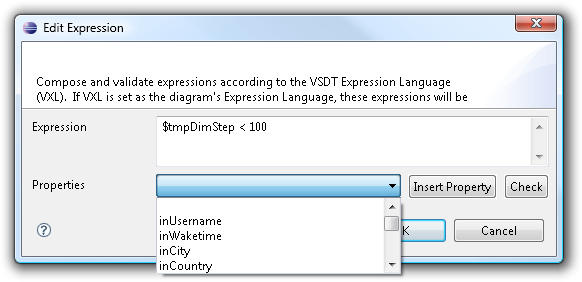
\includegraphics[width=.5\textwidth]{figures/features/editExp.png}
	\caption{The Edit Expression Dialog.}
	\label{fig:editExp}
\end{figure}

Each text field referring to an Expression in the dialogs and property sheets of the VSDT provides a
small button for opening the Edit Expression Dialog, which can be seen in Figure~\ref{fig:editExp}.
This dialog not only provides a large text field for editing the Expression, but also a list of all
Properties visible in the scope of the element owning the Expression, which can be selected from the
list and inserted into the expression. Further, the \emph{Check} button can be used to validate the
Expression, which will check both the syntax and the availability of the variables used in the
expression.

\emph{Note} that there is no type checking yet. However, this feature is on the agenda, and will be
implemented as soon as possible.


\section{Service Parameter Assignments}

While the \emph{Organize Assignments Dialog} provides means for organizing all types of Assignments,
it can be quite weary to make the assignments to a service call, passing a number of values to the
service's input parameters and storing its results in other local variables. Moreover, this is a
common source for mistakes, like selecting the wrong assign time, or missing an important input
parameter. Using the \emph{Parameter Assignments Dialog} this task can be facilitated in many ways.

\begin{figure}[ht]
	\centering
	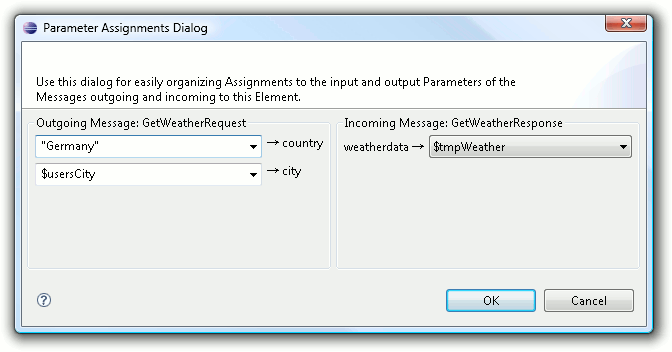
\includegraphics[width=.6\textwidth]{figures/features/paramAssign.png}
	\caption{Parameter Assignments Dialog}
	\label{fig:paramAssign}
\end{figure}

This dialog is available for all Activities and Events sending or receiving messages, such as the
Message Event and Send, Receive, Service and User Activity. Provided that the Implementation and the
input and output Messages for that service are specified, the dialog displays a drop-down menu for
each of the incoming and/or outgoing Messages' Properties. The values set in these lists will then
be used for the Assignments to the input and output parameters. For the outgoing message, arbitrary
expressions can be inserted, while the parameters of the incoming message can only be assigned to a
local Property. If more specific Assignments are needed, the dialog can still be used for generating
stubs for those Assignments, which then can be refined in the \emph{Organize Assignments Dialog}.
Further, the dialog will notify the user if there are input parameters that have no value assigned
to them.


\section{Inserting Elements and Patterns}
\label{sec:user_features_patterns}

By right-clicking on a Sequence Flow the \emph{Insert...} menu can be reached. Here it is possible
to insert a new element in between the source and the target of that Sequence Flow, which is very
useful for extending existing diagrams. The existing sequence Flow will be reoriented to the new
element, preserving existing attributes such as the condition, and a second Sequence Flow is drawn
from the new element to the existing Sequence Flow's former target.

Apart from simple elements such as Activities, Intermediate Events and Gateways, it is also possible
to insert complex workflow patterns, such as a split/merge block or a loop. This does not only
greatly reduce the time needed for the diagram creation\footnote{Reducing the pure editing time by
up to 70\% according to ~\cite{gschwind2008applying}.}, but also ensures that the workflow is
correct (Referred to as ``correctness by construction'').

\emph{Note} that by now the layout of the diagram will not be adapted to the newly inserted
elements, thus the user will have to rearrange the surrounding elements to make room for the new
nodes.

\section{Appending Flow Objects}
Similarly to the \emph{Insert} Actions, the \emph{Append} Actions can be used for quickly appending
new Flow Objects after existing ones. It can be reached through a Flow Object's context menu, or --
more conveniently -- by using the keyboard shortcuts \texttt{Ctrl+Shift+(A|G|I|E)} for appending
Activities, Gateways, Intermediate and End Events. Thus, after the first Start Event has been
placed, the basic workflow can quickly be assembled using only the Append action and the TAB key to
navigate between the existing nodes.

\section{Connecting Flow Objects to a Sequence}
Further, a group of Flow Objects can be selected and connected with Sequence Flows using
\emph{Connect to Sequence} Action or the keyboard shortcut \texttt{Ctrl+Shift+C}. The Flow Objects
will be connected in the order they have been selected. Therefore they should be selected one by one
(holding down the Shift or Ctrl key), and not using a selection margin.


\section{Model Validation}
\label{sec:user_features_validate}

VSDT provides two sorts of validation: Validation of BPMN constraints, and structural validation.

\paragraph{Validation of Constraints}
BPMN diagrams can be checked to conform to the constraints given in the BPMN specification by
selecting \emph{Diagram $\rightarrow$ Validate} from the menu or by clicking the checkmark icon in
the tool bar. Afterwards errors will be listed in the problem view. Additionally, faulty or
otherwise problematic elements will be marked with a respective icon in the process graph.

\paragraph{Structural Validation}
Besides the individual elements, also the structures in which these elements are connected are
important. For checking the structure of the process, open the Structure View (see Section
\ref{sec:user_perspective_strucView}) and click the \emph{Structurize} button. This will trigger the
same Structure Mapping used in the actual transformations and display the result, i.e. a structured
form of the process, featuring elements such as sequences and blocks. While the structured model
might be a bit cumbersome to read, it gives evidence of the structure that will be recognized from
the process, and if this is not the structure you intended you should consider restructuring the
process.


\section{Text Generation}
\label{sec:user_features_text}
 
The VSDT features a powerful transformation of the Business Process Diagram to natural language
text. Currently only English text is supported, but other languages may be included in the future,
as well. The output text can have different formats, e.g. plain text, HTML or Latex, which to use
can be selected in the Export Wizard. While this feature is yet at an early stage, it can already be
used for quickly generating documentation for those who can not read the process diagrams or for
media where they are difficult to present, e.g. in a talk. Emphasis has been laid on preserving the
process structure as much as possible in the text, e.g. using indentation. Further a number of
randomly selected redundant terms is used to increase the linguistic diversity of the resulting
text.


\section{Simulation and Interpretation}
\label{sec:user_features_sim}

BPMN diagrams created with the VSDT can be simulated and interpreted using the built-in process
interpreter (see Section~\ref{sec:user_perspective_simView}). For starting a simulation, first
switch to the BPMN diagram you want to simulate. Open the \emph{Process Interpreter} view and click
the \emph{Start} button. For each Pool in the diagram, the view will show those Activities that are
currently \textsc{active} or \textsc{ready}. For advancing a step in the simulation, expand a Pool
and double-click one of the listed elements, that is the Flow Objects currently being ready, e.g.\
Start Events. For more control, you can also select one of \emph{Step Over}, \emph{Step Into} or
\emph{Step Out}. Hit the Stop button for ending the simulation and removing the markers from the
diagram editor view. In the diagram itself, the Flow Objects are annotated with a marker symbol
representing their state (see Table~\ref{tab:markerColors}).
\begin{table}[ht]
	\centering
	\caption{Mapping of Marker Colors to Flow Object States}
	\label{tab:markerColors}
	\begin{tabular}{|l|l|}
		\hline
		Yellow & Ready for execution             \\
		Blue   & Currently active / executing    \\
		Green  & Executed succesfully            \\
		Red    & Execution failed or interrupted \\
		None   & Not yet executed or ready; idle \\
		\hline
	\end{tabular}
\end{table}

Once the simulation is running, the user can \emph{Step Over}, \emph{Step Into} and \emph{Step Out}
of Flow Objects. Stepping into a Flow Object is particularly interesting for Activities with
attached Event Handlers or Embedded Subprocesses, for which it is the default behaviour. Different
kinds of interpretations are available (or planned for the future):
\begin{itemize}
	\item \emph{Manual Simulation}: Here, the user is asked which way to proceed when coming to a
	branching point. This mode is intended for presentation, but also for detecting e.g.\ deadlocks
	or other kinds of structural conflicts.
	\item \emph{Interpretation}: In this mode, Expressions used for instance in Assignments and
	Conditions are evaluated\footnote{Note that only Expressions given in the VSDT Expression
	Language can be automatically evaluated, and that by now only simple data types are supported.}
	and stored, so that the process will automatically decide how to proceed at a branching point.
	Still, the user has to provide initial parameters and return values for service calls. This mode
	is especially useful for testing the various Conditions and Assignments. \emph{(work in
	progress)}
	\item \emph{Execution}: This mode integrates with the Rich Service Directory (RSD), meaning that
	in addition to the \emph{Interpretation} mode services will be invoked using the RSD and their
	return values will be bound to the respective process properties. Thus the user just has to
	provide the initial parameters of the process itself. Apart from testing the interworking of the
	several services in the process, this mode can also be used for actually executing and
	monitoring the process. \emph{(future work)}
\end{itemize}


\section{Structure-Based Layout}
\label{sec:user_features_layout}

The Structure Mapping can also be used for calculating the layout of the BPMN diagrams. Compared to
the layouting algorithm provided by GMF, this proves especially useful for diagrams containing
upstream loops. Still, since the structure-based layout is still in an early stage, the default
layouting algorithm still is the one provided by GMF. The structure-based layout can be reached via
the Structure View (see Section~\ref{sec:user_perspective_strucView}).


\section{Import and Merging of Process Diagrams}
\label{sec:user_features_merging}

VSDT diagrams can be imported into and merged with each other. While basically this feature can be
used for merging any two or more diagrams, it is most useful for merging diverging versions of the
same process diagram, having a common ancestor.

After selecting \emph{Import other VSDT diagrams} from the Import menu, select one or more diagrams
to import \emph{from} and one diagram to import \emph{into}. You can also check whether to create a
backup of the original target file (recommended), and whether the layout should be imported, too, or
only the model data, and whether the algorithm should try to merge identical elements. The latter,
of course, only makes sense if the source and target files are different revisions of the same 
process diagram.

The merging algorithm works by recursively comparing the IDs of the objects to be merged, so these
should not be changed in different revisions. Also there are still some issues with conflicting
changes, so one should always be sure to create a backup and possibly use a \texttt{diff} tool to
check whether the changes to the file's XML source look plausible.


	\chapter{Preferences}
\label{sec:user_preferences}

This chapter will explain the several preferences that can be set for configuring
the VSDT for your personal needs.

The preference pages can be accessed by navigating to \emph{Window $\rightarrow$
Preferences\dots} in the menu and selecting \emph{VSDT Diagram} from the list.
The following sections will each explain one of the pages.


%%%%%%%%%%%%%%%%%%%%%%%%%%%%%%%%%%%%%%%%%%%%%%%%%%%%%%%%%%%%%%%%%%%%%%%%%%%%%%%%

\section{Basic GMF Settings}
\label{sec:user_preferences_gmf}

These settings are for improving performance by deactivating certain features of
the GMF runtime, or for setting the default colors and fonts for certain diagram
elements.  As these features are self-explaining we will not go further into
detail here.


%%%%%%%%%%%%%%%%%%%%%%%%%%%%%%%%%%%%%%%%%%%%%%%%%%%%%%%%%%%%%%%%%%%%%%%%%%%%%%%%

\section{VSDT Settings}
\label{sec:user_preferences_vsdt}


\subsection{General}
\begin{itemize}
	\item \textbf{Author} sets the default author for all new Business Process
	Diagrams created.
	
	\item \textbf{Enable Modeling Assistance} turns GMF's modeling assistance on
	or off (see Section \ref{sec:user_features_assistance}).
\end{itemize}	


\subsection{Appearance}
\begin{itemize}
	\item \textbf{Enable Activity Icons} activates additional markers placed in
	the corners of Activities.  These markers use intuitive symbols to indicate
	the Activity's type and whether the Activity has any Assignments and/or
	Properties.
	
	\item \textbf{Use Additional Colors} helps to distinguish the several diagram
	elements by the use of colors.
	
	\item \textbf{Show XOR-Marker for new Gateways} sets whether to display the
	cross-marker for new XOR gateways.
	
	\item \textbf{Meta Diagram Style} lets you choose between a notation similar
	to UML use cases or BPMN 2.0 communication diagrams for the VSDT's entry
	diagrams.
\end{itemize}


\subsection{Connections}
Here you can select the drawing style for Sequence Flows, Message Flows and
Associations.

\emph{Note} that both the Enable Activity Icons and the Use Additional Colors
settings take effect only after closing and reopening a given Business Process
Diagram file.


	\chapter{Model Transformation}
\label{sec:user_trafo}

The core of the Visual Service Design Tool clearly is the transformation to
executable code.  While by now the transformation to BPEL is the only one that
can be conveniently used in practice, there are currently several other
transformations under development.

For directions on how to invoke the transformation please refer to
Section~\ref{sec:user_tut_export}.


%%%%%%%%%%%%%%%%%%%%%%%%%%%%%%%%%%%%%%%%%%%%%%%%%%%%%%%%%%%%%%%%%%%%%%%%%%%%%%%%

\section{Understanding the Transformation Framework}
\label{sec:user_trafo_intro}

This section will provide a brief introduction in the basics of the transformation
framework.  The transformation framework has been designed from the very beginning
to be as \emph{extensible} and \emph{reusable} as possible.  For that purpose the
process of transformation has been subdivided into several stages, which are
sequentially applied to the input model:
\begin{enumerate}
	\item In the \emph{Validation} stage, all identifiers are validated to contain
	only characters that are legal with respect to the given target language.
	Further, the validation will check if each element needed is in place and
	providing clear error messages in case something is missing.
	
	\item The intent of the \emph{Normalisation} stage is to put the process
	diagram in a uniform form, and to transform it to a semantically equivalent
	representation of the diagram following more strict constraints than those
	given in the BPMN specification.
	
	\item In the \emph{Structure Mapping} stage, the model is searched for graph
	patterns which are semantically equivalent to block structures.  When such
	patterns are found, they are replaced with a special structured element, until
	the entire process within each Pool has been reduced to a single complex
	element, e.g.\ a sequence, or until it can not be reduced any further due to
	structural flaws.
	
	\item In the \emph{Element Mapping} stage, the several BPMN elements are
	mapped to their counterparts in the target language, e.g.  BPEL or JIAC
	(Section~\ref{sec:user_trafo_bpel} and~\ref{sec:user_trafo_jiac}).
	
	\item In the \emph{Clean Up} stage, a set of rules is applied on the newly
	created target model, improving the readability of the generated code and
	removing redundancies.
\end{enumerate}

A simple example of the consecutive execution of normalisation and structure
mapping can be seen in Figure~\ref{fig:norm_struc}.

\begin{figure}
	\centering
	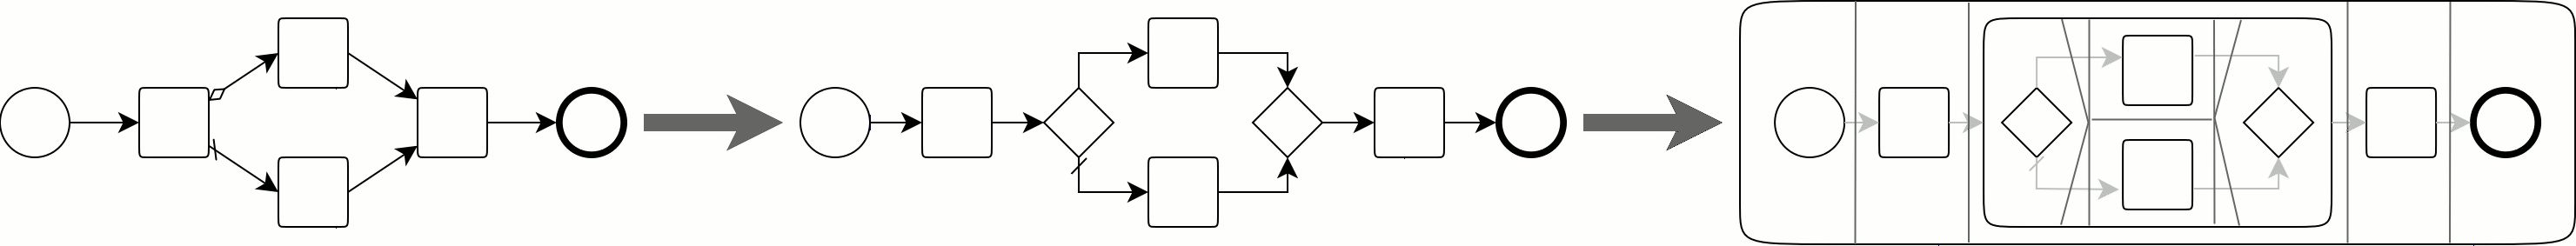
\includegraphics[width=\textwidth]{figures/trafo/norm_struc_2.png}
	\caption{Simple example of normalisation and structure mapping.}
	\label{fig:norm_struc}
\end{figure}


\subsection{Transformation of Expressions}

Besides the actual workflow, Expressions that are used in assignments and
conditions have to be translated, too.  This can be done only if the Expression
Language is set to ``VSDT Expression Language'' or ``VXL''.\footnote{The Expression
Language can be set either globally in the Diagram properties or individually for
each Expression.} If then the \emph{Translate Expression} option is checked in
the Export Wizard (see Figure~\ref{fig:trafo_wiz}) these expressions will be
parsed and, if possible, translated to the respective target language.

\begin{figure}
	\centering
	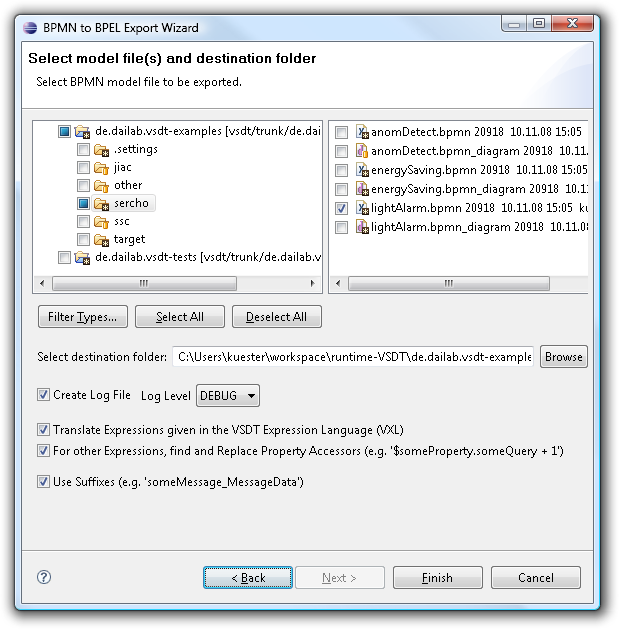
\includegraphics[width=.5\textwidth]{figures/features/exportWiz.png}
	\caption{BPEL Export Wizard with Expression Translation checked.}
	\label{fig:trafo_wiz}
\end{figure}

Still there may be cases when VXL does not have enough expressive power.  In this
case the option can be disabled (or the Expression Language can be changed) and
the \emph{Replace Property Accessors} option can be checked.  In this case, the
Expressions will only be scanned for Property Accessors using VXL (e.g.
\texttt{\$foo.bar}) which will then be translated to the syntax of the target
language.  Thus, the simple VXL variables can be embedded in expressions of
another language.  For instance, in the case of BPEL, an expression like
\texttt{\$foo.bar + 1}, might be changed to \texttt{bpws:getVariableData(
'Proc\_ProcessData','foo','bar')+1}.  Thus the user does not have to care about
the way Properties are aggregated to variables in the transformation to that
language but can simply use a Property's name.

Finally, when Properties are given one of VXL's predefined basic data types (e.g.
\texttt{string}, \texttt{boolean}, etc.), where will be translated to the
respective basic types of the target language, e.g. \texttt{xsd:string} and
\texttt{xsd:boolean}.


%%%%%%%%%%%%%%%%%%%%%%%%%%%%%%%%%%%%%%%%%%%%%%%%%%%%%%%%%%%%%%%%%%%%%%%%%%%%%%%%

\section{Transformation Implementations}
\label{sec:user_trafo_impl}

The following sections describe in short the various transformations that have
already been implemented.


\subsection{Transformation to Text}
\label{sec:user_trafo_text}

See Section~\ref{sec:user_features_text}.


\subsection{Transformation to BPEL}
\label{sec:user_trafo_bpel}

The transformation to BPEL presented in this work covers nearly the entire mapping
as given in the BPMN specification~\cite[Appendix A]{omg2009bpmn}, including event
handlers, inclusive \textsc{or} and event-based \textsc{xor} Gateways, just to
name a few.

\paragraph{Export}
Nevertheless there are some elements for which the mapping is not given very
clearly, such as \textsc{timer} Start Events, independent Sub Processes or
multi-instance parallel loops.  While these elements will be transformed as
described in the specification, the resulting BPEL processes will require some
amount of manual refinement.  Besides the BPEL process files a WSDL definitions
file is created, holding the message types derived from the process properties
and the input and output messages and interfaces (port types) for the several Web
services being orchestrated by the process.  Still, the WSDL's binding and service
blocks and necessary schema types, if any, can not be generated automatically
yet, due to insufficient information in the source model.

In the validation, all identifiers are tested to contain only characters that are
legal with respect to BPEL, and all expressions used e.g.\ in Assignments and
loop conditions are translated to XPath, if possible.  Properties are aggregated
to one variable per Process or Message, for instance, if a Process \texttt{Proc}
has a Property \texttt{foo}, \texttt{foo} will be a Part of Variable
\texttt{Proc\_ProcessData}.

\paragraph{Import}
The Import from BPEL to BPMN is still at an early stage.  While basic control
flow can be imported, there are still problems e.g. with event- and fault handlers.
Further one should be aware that the export to BPEL does not preserve all
information in the BPMN diagram, thus diagrams re-imported after being exported
to BPEL will most likely be less readable than before, although they may be
semantically equivalent.


\subsection{Transformation to JIAC}
\label{sec:user_trafo_jiac}

Concerning our goal of transforming BPMN diagrams to multi-agent systems (MAS)
the work is still at an early stage.  First, a \emph{normal form} for BPMN diagrams
has been investigated, to facilitate the mapping~\cite{endert2007towards}.  Later,
the first steps of the actual mapping have been developed, basically mapping Pools
to agents, Processes and Flow Objects to the agents' plans and the control flow,
and Message Flow to the exchange of messages between the agents~\cite{endert2007mapping}.

\paragraph{Export}
A prototypic transformation targeting the agent framework JIAC V has already been
implemented.  In this transformation, the Participants diagram is translated to
an Agent World diagram, and the individual Business Processes are translated to
several JADL services.  As the theoretical part of the mapping is not yet fully
matured, there is still some work to do.  However, with the given transformation
framework every addition to the mapping can quickly be adopted.

The \emph{BPMN to JIAC Transformation} feature requires the \emph{JIAC Agent World
Editor} feature.


\subsection{Transformation to STP-BPMN}
\label{sec:user_trafo_stp}

Since BPMN does not provide a standardized interchange format, transferring a
diagram from one editor to another is difficult.  For that reason the VSDT provides
a Transformation to the popular Eclipse STP-BPMN Editor.  Thus one can export a
Diagram to STP-BPMN and carry it to a colleague using that editor, or someone
formerly using the STP editor can import his existing files when changing to the
VSDT.

\paragraph{Export}
The export to STP is nearly complete.  The only elements that are not mapped are
Lanes, which is because the STP editor is encountering problems when initializing
the diagram files containing Lanes.  Alas, the same also applies to Embedded
Subprocesses, as there are problems opening those diagrams.  However, this is a
problem with the STP editor that will get fixed soon.

\paragraph{Import}
The import from STP works very well, with the exception that, again, Lanes will
not be mapped. \emph{Note} that the transformation to STP will only create the
BPMN model files, but not the diagram files; those files, holding the graphical
information, have to be generated anew from the model file.  Thus, the transformation
does not preserve the layout of the diagrams.

The \emph{BPMN to STP-BPMN Transformation} feature requires the \emph{Eclipse SOA
Tools Project BPMN Editor} feature.


%%%%%%%%%%%%%%%%%%%%%%%%%%%%%%%%%%%%%%%%%%%%%%%%%%%%%%%%%%%%%%%%%%%%%%%%%%%%%%%%

\section{Limitations}
\label{sec:user_trafo_limits}

Although the transformation framework is quite powerful, it is important to
understand that there are still some limitations, both in the mapping of structures
and elements.

\begin{itemize}
	\item Given a well-structured workflow, the transformation will yield very
	good results.  However, as BPMN is more powerful that block-oriented languages,
	such as BPEL and JIAC, there will always be graph structures that can not be
	transformed to an equivalent program of the target language.  In that case
	the diagram should be manually restructured \emph{before} being exported.
	
	\item The mapping to BPEL is as complete as possible, according to the
	specification.  Still, there are some points in the specification that are
	missing, unclear or ambiguous.  The transformation to BPEL is implementing
	the specification in almost every detail, but regarding these elements a small
	amount of manual refinement may be necessary.
	
	\item The mapping to JIAC is still at an early stage.  JIAC models created
	with this transformation will require a large amount of manual work.
\end{itemize}

We are constantly investigating ways of extending both the quality of the element
mappings and the performance of the structure mapping.


%	\chapter{FAQ}
\label{sec:user_faq}

This chapter will give valuable advice on how to solve several tasks, solve problems, and answer
other questions related to the Visual Service Design Tool.


\section{How to...}
\label{sec:user_faq_howto}

\paragraph*{\dots draw Flow Objects on the Canvas?}
Although sometimes such diagrams can be seen, Flow Objects \emph{can not} be drawn on the canvas.
Instead, each Flow Object has to be contained in a Lane, and the Lane has to be inside of a Pool.
However, according to the specification one Pool per diagram may have an invisible border, which can
be set using the property sheets.

\paragraph*{\dots create an Embedded Sub Process?}
First, create a basic Activity. Then, in the Activity's property sheet, set the activity type to
\textsc{Embedded Sub Process}. Now you can resize the Activity/Sub Process to an appropriate size
and create further Flow Objects inside of it.

\paragraph*{\dots create an Intermediate Event on an Activity's boundary?}
For creating an Intermediate Event on an Activity's boundary, i.e. an event- or error handler, you
should select the Event type from the palette and click the Activity's label or boundary, and
\emph{not} the compartment. Alternatively, you can use the miniature palette that appears when
hovering the mouse over the Activity's label or boundary. Once created, the Intermediate Event can
be moved freely around the Activity's border.

\paragraph*{\dots draw Artifacts inside of a Pool?}
Contrary to Flow Objects, Artifacts can not be created inside of a Pool. However, you can create the
Artifact on the canvas and drag it over the Pool. But remember that the Artifact is \emph{over}, and
not \emph{in}, the Pool, so it will not be moved together with the Pool.

\paragraph*{\dots make Assignments to Message Parameters?}
The arguments and results of service invocations are being stored in the Properties of the input
Message and the output Message. So if a service is to be called with the argument "Hello World",
that value has to be assigned to the respective Property of the service's input Message using the
\emph{Organize Assignments Dialog} of the Activity calling the service. Note, that Assignments to
the input parameters have to be made \emph{before}, and Assignments storing the output parameters in
local variables have to be made \emph{after} the Activities execution. The Assign Time can be
specified in the Dialog, too. However, a more convenient way, and sufficient in most situations, is
to use the \emph{Parameter Assignments Dialog}, which will take care of most of these details. Of
course, the same applies to Message Events and Send and Receive Activities, as well.

%\paragraph*{\dots enter a Time Date value?}
%This value is expected in quite complex form, because it has to be processed by a parser. The value
%has to be in the form "yyyy-MM-dd'T'HH:mm:ss.SSSZ", e.g. "2007-02-12T14:53:00.000+0100" for Monday,
%the 12th of February 2007 at 14:53:00 CET.


\section{Frequently Asked Questions}
\label{sec:user_faq_faq}

\paragraph*{My diagram is broken. How can I fix it?}
In case the diagram is broken, it can be recreated from the model. In case you are using separate
files for semantic model and notational model, delete the diagram file \texttt{vsdt_diagram} and
create a new one by right-clicking the model file \texttt{vsdt} and selecting the respective menu
item. In case you are using one file for both semantic and notational model, \texttt{vsdtd}, open
the file in a text editor and remove the \texttt{notation:Diagram} elements (one for each diagram
contained in the file). Now rename the file to \texttt{vsdt} and initialize the diagram file (in
this case you can delete the model file afterwards, as the model has been copied to the diagram
file). In both cases, you will have to recreate the diagram's layout.


\section{Troubleshooting}
\label{sec:user_faq_trouble}

\paragraph*{I've drawn a legal Business Process Diagram, but when I try to export it the resulting
code is broken.}
The diagram has to be in a certain form so it can successfully be transformed. The diagram has to be
\emph{structured}. Primarily, there must not be blocks or loops with multiple entry or exit points.
Although the VSDT can handle some forms of slight unstructuredness, for best results you should
design your diagram in a way it can be mapped to a block-oriented language in a straight-forward
manner.

\paragraph*{I've created a Business Process Diagram using element XYZ, but in the resulting code
this element is missing.}
Not each single feature of BPMN can be taken into account in all of the transformations yet. For
those elements that can not be mapped, a no-operation element will be created in the target model,
such as a \verb|empty| Activity in BPEL or a \verb|logwarn| in JIAC. Be sure to substitute these
elements with a proper implementation after the transformation.


%	\part{Developer Notes}
	% plugins-ordnung
	% auflistung der wesentlichen erweiterungen
	% transformation framework
	% einzelne regeln beschreiben
	% how to write a new trafo

%	\part{Appendices}
	\begin{appendix}
		\chapter{The Business Process Modelling Notation}
\label{sec:bpmn}

%%% aus meiner Diplomarbeit

% introduction
The \emph{Business Process Modelling Notation(BPMN)} was first published by the
BPMI and has then been adopted by the OMG (Object Management Group)~\cite{omg2009bpmn}.
The goal of the development of BPMN was to create a standardized modeling notation
for business processes, thus reducing the confusion created by dozens of proprietary
business process notations.  A brief introduction to BPMN is given for instance
in~\cite{white2004introduction}.

% basic elements
There are four basic categories of element types in the notation: Flow Objects
(Events, Activities and Gateways), Connecting Objects (Sequence Flows, Message
Flows and Associations), Swimlanes (Pools and Lanes) and Artifacts (Data Objects,
Groups and Annotations).

\begin{figure}[ht]
	\centering
	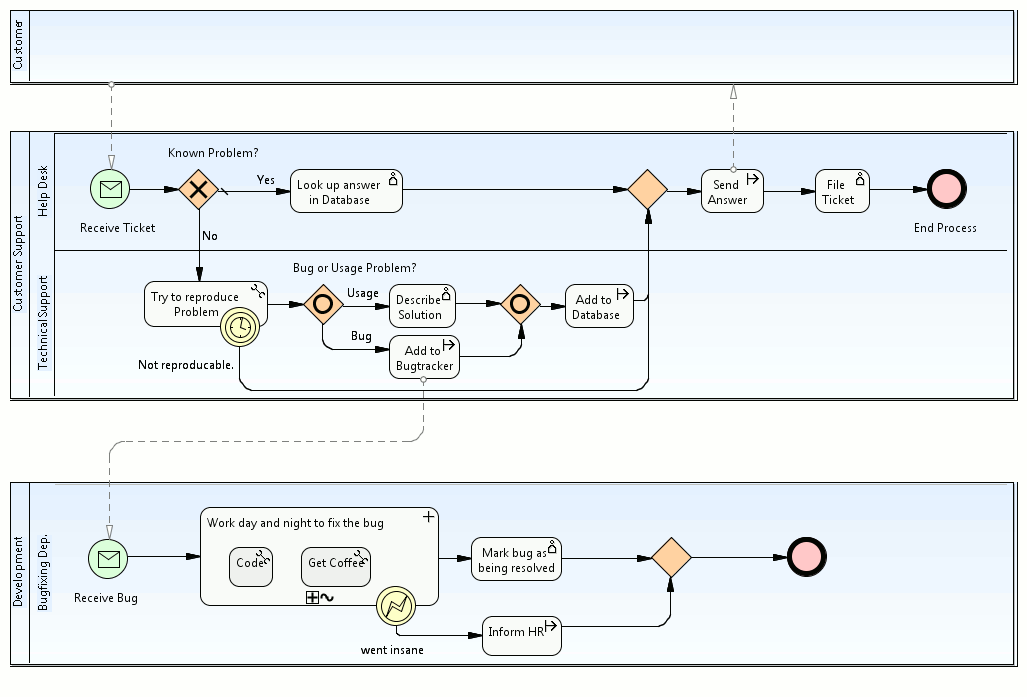
\includegraphics[width=.8\textwidth]{figures/bpmn/example.png}
	\caption{Business Process Modelling Notation Example Diagram}
	\label{fig:bpmn_example}
\end{figure}

Figure \ref{fig:bpmn_example} shows a simple example diagram.  The elements are
quite self-descriptive and most of them are already known from other notations,
so the basics of the BPMN are readily understandable for all business analysts,
architects and developers and even for non-experts.  At the same time BPMN provides
a large variety of subtypes for each of the Flow Objects and every element type
is enriched with many non-graphical attributes, making the models sufficiently
detailed for being exported to executable languages while keeping the visual
notation concise and understandable.

A problem with BPMN is that it is mainly a \emph{notation}.  Although the
specification describes many non-graphical attributes and a mapping to a formal
language, it neither states an exchange format, like an XSD, nor clear semantics
for all of the elements.  Still the Business Process Modeling Notation can be
used throughout the entire software engineering life-cycle, from a simplified model
at the requirements analysis up to a highly detailed model that can be used for
generating code for an executable language.


%%%%%%%%%%%%%%%%%%%%%%%%%%%%%%%%%%%%%%%%%%%%%%%%%%%%%%%%%%%%%%%%%%%%%%%%%%%%%%%%

\section{BPMN Elements}
\label{sec:bpmn_elements}

This section is intended to give a brief introduction of each of the basic element
groups:

\begin{itemize}
	\item \textbf{Flow Objects}: Events, Activities, and Gateways
	\item \textbf{Connecting Objects}: Sequence Flows, Message Flows and Associations
	\item \textbf{Swimlanes}: Pools and Lanes
	\item \textbf{Artifacts}: Data Objects, Groups and Annotations
\end{itemize}

\subsection{Flow Objects}

The category of \emph{Flow Objects}, the most important elements in BPMN, is made
up of \emph{Events}, \emph{Activities} and \emph{Gateways}.  All Flow Objects are
held in Lanes (see below).

\textbf{Events} are things that \emph{happen}, like a message arriving, an alarm,
or an error, and often they mark the beginning and the end of the process.  The
graphical notation is a circle.  They are subdivided into \emph{Start Events},
\emph{Intermediate Events} and \emph{End Events}, which determines the circle's
border (see figure \ref{fig:events}).

\begin{figure}[ht]
	\centering
	
\includegraphics[width=.75\textwidth]{figures/bpmn/events.png}
	\caption[BPMN Event types]{BPMN Event types.  From left to right: Start Event,
	Intermediate Event, End Event}
	\label{fig:events}
\end{figure}

Further all three Event types have a variety of subtypes which will determine
e.g. a Start Event's \emph{trigger} and an end Event's \emph{result}.  Each of
these subtypes can be distinguished by a different icon in the center of the Event
figure (see figure \ref{fig:triggers}) and results in a number of attributes to
be set for the Event.

\begin{figure}[ht]
	\centering
	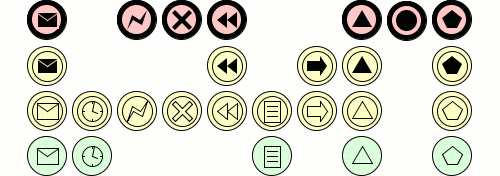
\includegraphics[width=.75\textwidth]{figures/bpmn/triggers.png}
	\caption[BPMN Event sub types]{BPMN Event sub types.  From left to right:
	Message, Timer, Error Cancel, Compensation, Rule, Link, Signal, Termination,
	Multiple}
	\label{fig:triggers}
\end{figure}

Basically, an \textbf{Activity} is something that is \emph{done}.  Activities
subdivide in \emph{Tasks}, which are atomic Activities, and \emph{Sub Processes},
which are composite Activities.  The graphical notation for an Activity is a
rounded rectangle with the Activity's name inside of it.  Sub Processes are marked
with a small $ \boxplus $ sign on the bottom line (see figure \ref{fig:activities}).

\begin{figure}[ht]
	\centering
	
\includegraphics[width=.75\textwidth]{figures/bpmn/activities.png}
	\caption[BPMN Activity types]{BPMN Activity types.  From left to right: Task,
	Subprocess}
	\label{fig:activities}
\end{figure}

Like Events, Activities also have some specializations, each one with special
attributes: They can be for instance a \emph{Send} or a \emph{Receive} Task, stand
for some \emph{Manual} work to be done, execute a \emph{Script} or represent the
call to a whole other business process, just to name a few.  All of these subtypes
have the same graphical representation, but modelers and modeling tools are
free to extend the diagrams with additional markers for the subtypes.

What makes Activities stand out from the other Flow Objects is that they can
\emph{loop}.  Although in BPMN loops also can be defined by simply connecting a
Sequence Flow to an upstream Flow Object, which might be easier to understand by
non-experts, it's seen as better style to use looping Activities, where
applicable.  A looping Activity is marked with a small counter-clockwise arrow on
its bottom line.

\textbf{Gateways} provide wide capabilities in modeling all kinds of splitting
and merging behavior.  Figure \ref{fig:gateways} shows the different kinds of
Gateways.  Depending on whether the Gateway has multiple incoming or outgoing
Sequence Flows --- or even both --- it has different semantics, like forking
and/or joining the flows.  However, Gateways are not the only way for modeling
forking and joining of flows: In some cases the same semantics can be reached
by omitting the Gateway and connecting multiple Sequence Flows directly to an
Activity (but not Events).  However, this should also be considered bad style.

\begin{figure}[ht]
	\centering
	
\includegraphics[width=.75\textwidth]{figures/bpmn/gateways.png}
	\caption[BPMN Gateway types]{BPMN Gateway types.  From left to right: Data-based
	XOR (with and without marker), Event-based XOR, Inclusive OR, Complex, AND}
	\label{fig:gateways}
\end{figure}


\subsection{Connecting Objects}

The most important connections are \emph{Sequence Flows} and \emph{Message Flows}.
Sequence Flows represent the flow of control and connect Flow Objects within a
Pool in the order of execution.  Message Flow represents messages --- not
necessarily data --- being exchanged exclusively between Pools.  See figure
\ref{fig:connections} for the connections' graphical notation.

\begin{figure}[ht]
	\centering
	
\includegraphics[width=.75\textwidth]{figures/bpmn/connections.png}
	\caption[BPMN Connection types]{BPMN Connection types.  From left to right:
	Sequence Flow, Message Flow, Association}
	\label{fig:connections}
\end{figure}

The third connection, the \emph{Association}, is mainly used for documentation
purposes, for instance to connect a Text Annotation to a Flow Object that needs
further explanation.  Still there is an exception to this rule: For connecting a
compensating Activity to a compensation Event an Association is used instead of
a Sequence Flow.  An Association's arrow heads are optional.


\subsection{Swimlanes}

Swimlanes can be \emph{Pools} and \emph{Lanes}.  Each Pool represents one
Participant in the business process, while Lanes are used to partition a Pool.
Doing so each of a company's departments could be represented by a Lane while the
Pool stands for the company itself.  However, the semantics of both Pools and
Lanes is not entirely fixed.  Typically Swimlanes are oriented horizontally,
but may be oriented vertically, too.  Further, Lanes may cross or contain other
Lanes, but those techniques are poorly documented and seldom used.  Figure
\ref{fig:swimlanes} shows a small horizontally oriented Pool containing two empty
Lanes.

\begin{figure}[ht]
	\centering
	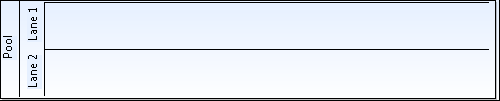
\includegraphics[width=.75\textwidth]{figures/bpmn/swimlanes.png}
	\caption[BPMN Swimlanes]{BPMN Swimlanes. A Pool with two Lanes}
	\label{fig:swimlanes}
\end{figure}


\subsection{Artifacts}

The main purpose of \emph{Artifacts} is documentation.  However, like Associations,
in some situations they can have semantics, e.g. when a \emph{Data Object} is
referenced by an Activity as input.  Data Objects represent everything that can
be input or output of some Activity.  In most cases this will be a file, or some
piece of data, but since Activities can be \emph{Manual Tasks}, too, a Data Object
could also stand for something physical.

The other two Artifacts, \emph{Group} and \emph{Text Annotation}, are solely used
for documentation.  See figure \ref{fig:artifacts} for their graphical notation.

\begin{figure}[ht]
	\centering
	
\includegraphics[width=.75\textwidth]{figures/bpmn/artifacts.png}
	\caption[BPMN Artifacts]{BPMN Artifacts.  From left to right: Data Object,
	Group, Text Annotation}
	\label{fig:artifacts}
\end{figure}

The specification states that this category may be extended by proprietary
Artifacts which could have more semantics, too.  This way BPMN can be extended
with new elements to represent concepts that were not considered in the original
specification.


%%%%%%%%%%%%%%%%%%%%%%%%%%%%%%%%%%%%%%%%%%%%%%%%%%%%%%%%%%%%%%%%%%%%%%%%%%%%%%%%

\section{Levels of Complexity}
\label{sec:bpmn_complexity}

% drei layer
BPMN can be seen as having at least three levels of complexity.

\begin{enumerate}
	\item Basic Types: All diagrams are made up of the basic elements of the four
	categories: Events, Activities, Gateways, Connections, Pools and Artifacts.
	These can be understood easily even by non-experts.
	
	\item Subtypes: The Flow Objects each have several subtypes, e.g.  Timer
	Events, Receive Tasks and Inclusive Gateways.  Using the same shapes as the
	basic elements enriched with some additional graphical information, like an
	icon, the symbol's basic type can be clearly identified by non-experts while
	providing additional visual information for the professionals.
	
	\item Attributes: Each of the BPMN element types provides a large number of
	both primitive and complex attributes.  While some of these attributes are
	visible in the diagram, like a flow object's name or subtype, most are
	non-graphical.  These attributes enrich the diagram with the formal semantics
	necessary for the export to an executable language while not polluting the
	visual notation with too many details.
\end{enumerate}

% notation teils ohne semantik (message flows)
If the process shall be mapped to a executable language the third level is very
important: Not only does it give values for many attributes that otherwise would
have to be set manually.  Some of the visual elements of the BPMN do not have
semantics ``on their own''.  Message Flows for example do \emph{not} have a
mapping to WS-BPEL.  Instead the source Activity has to be of type \texttt{Send}
and the target Activity of type \texttt{Receive}, and both have to reference the
same non-graphical \texttt{Message} element.  This is necessary in cases when the
communications partner is not in the same diagram and thus a Message Flow can not
be drawn.

Of course it is free to the designers of new mappings to map the Message Flow, if
it is available, without insisting on the existence of the non-graphical Message
element.


%%%%%%%%%%%%%%%%%%%%%%%%%%%%%%%%%%%%%%%%%%%%%%%%%%%%%%%%%%%%%%%%%%%%%%%%%%%%%%%%

\section{Export and Code Generation}
\label{sec:bpmn_export}

One of the main purposes of the Business Process Modelling Notation is to provide
a graphical process notation that can be used to generate executable code from it.

A mapping to WS-BPEL is given in the BPMN Specification.  As a matter of fact,
BPMN has been tailored for the mapping to WS-BPEL, which can be seen in many
attributes which are needed only for the mapping.  Most of these attributes can
be reused for mappings to other languages, too, e.g. such common concepts as
properties and assignments.

On the other hand BPMN has more expressive power than BPEL.  A diagram in BPMN is
a directed graph, while BPEL, and in fact most other executive languages as well,
are block oriented, making the export to a semantically equivalent program
complicated and in some cases impossible.  Numerous papers have been written on
how to identify block structures within a BPMN diagram or how to alter an existing
diagram to conform to block structure.  However, not every diagram can be
refactored like that.

While the basic elements such as Flow Objects should neither be altered nor
extended by new elements, the BPMN Specification encourages the introduction of
new, domain-specific Artifacts to be used in mappings to executable languages
other than BPEL.  These elements can be associated with the original BPMN elements
and represent concepts that were not considered in the original BPMN specification.


		
\chapter{The VSDT Expression Language (VXL)}
\label{sec:vxl}

The BPMN standard does not specify an expression language to be used. Instead, it is assumed that
the language of the target framework is used, e.g. XPath. However, in a tool that provides
transformations to various target frameworks this is not an option. While the diagram structure
could be translated to the syntax of the target system, the expression, given that they are written
in an unknown language, could not -- although all those languages might be very similar. To address
this flaw, the VSDT comes with its own, very simple expression language, the \emph{VSDT Expression
Language}, or VXL for short.


\section{Language Features and Syntax}

The VSDT Expression language has been designed to be the greatest common divisor of the expression
languages used in the target frameworks. Thus, most expressions can be given using VXL, in which
case they can be validated and -- more importantly -- parsed and translated to the respective
expression languages used in the target frameworks.

Below, the complete syntax of VXL is given. As can be seen, it is not much different from that of
other languages. Variables have to be the name of a Property in the scope of the owner of the
Expression. The Variable may be followed by one or more accessors, e.g. for access to an array
element (e.g. \verb|foo[2]|) or a field (e.g. \verb|foo.bar|), or combinations thereof (e.g.
\verb|foo[n+1].bar|); of course accessors can only be used if the target language and data type
supports them. An explanation of the various operations and comparisons can be found in
Table~\ref{tab:vxl_op}.

\begin{verbatim}
Term:           Head (Tail)?;
Head:           BracketTerm | Negation| Minus | Atom;
Tail:           Operator Term;
BracketTerm:    "(" Term ")";
Negation:       "not" Head;
Minus:          "-" Head;
Atom:           Value | Variable;
Variable:       ID (Accessor)?;
Accessor:       ArrayAccessor | FieldAccessor;
ArrayAccessor:  "[" Term "]" (Accessor)?;
FieldAccessor:  "." ID (Accessor)?;
Value:          STRING | INT | FLOAT| "true" | "false" | "null";
Operator:      "<" | "<=" | "==" | "!=" | ">" | ">=" | 
                "+" | "-" | "*" | "/" | "%" | "and" | "or" | "++";
\end{verbatim}


\begin{table}[htbp]
\centering
	\caption{VXL Operations and Comparisons}
	\begin{tabular}{r||lc}
		             & \textbf{Name}        & \textbf{Symbol} \\
		\hline
		Operations   & Addition             & \verb_+_	      \\
		             & Subtraction         & \verb_-_	      \\
		             & Multiplication       & \verb_*_        \\
		             & Division             & \verb_/_        \\
		             & Modulo               & \verb_%_        \\
		             & Concatenation        & \verb_++_       \\
		             & Logical \textsc{AND} & \verb_and_       \\
		             & Logical \textsc{OR}  & \verb_or_       \\
		             & Logical \textsc{NOT} & \verb_not_       \\
		\hline
		Comparisons & Equal                & \verb_==_       \\
		             & Not Equal            & \verb_!=_       \\
		             & Lesser               & \verb_<_        \\
		             & Lesser or Equal      & \verb_<=_       \\
		             & Greater              & \verb_>_        \\
		             & Greater or Equal     & \verb_>=_
	\end{tabular}
	\label{tab:vxl_op}
\end{table}

		
\chapter{Changelog}
\label{sec:changelog}

\paragraph{Version 1.3.1}
\begin{itemize}
	\item Interpreter: fixed evaluation priority in expressions, e.g.\ multiplication vs.\ addition
	\item \textbf{merging of different versions of a VSDT diagram}
	\item started Data Type Management
\end{itemize}

\paragraph{Version 1.3.0}
\begin{itemize}
	\item \textbf{switched to Eclipse 3.5}
	\item support for Conversation Diagrams (BPMN 2.0)
	\item \textbf{using one file for both semantic model and notational model}
	\item creation of diagram files (not only model files) on export and import
	\item export of BPMN diagrams with multiple start events to JIAC is now possible
	\item \textbf{added Connect to Sequence Action} for quick assembling of core process
	\item preferences can be used to deactivate the GMF modeling assistant
\end{itemize}

\paragraph{Version 1.2.2}
\begin{itemize}
	\item \textbf{Structure-based layout of BPMN diagrams}
\end{itemize}

\paragraph{Version 1.2.1}
\begin{itemize}
	\item \textbf{Export to JIAC V / JADL, integration with JIAC Agent World Editor}
	\item improved Pool / Lane visuals
	\item \textbf{added Append Node actios} for quick keyboard-based assembly of process diagrams
	\item added translation of basic data types, such as integer, string, etc.
	\item \textit{suspended support for JIAC IV and RSD}
\end{itemize}

\paragraph{Version 1.2.0}
\begin{itemize}
	\item \textbf{new diagram type: VSDT Meta Diagram (similar to UML usecases)}
	\item some more changes to the meta model
\end{itemize}

\paragraph{Version 1.1.3}
\begin{itemize}
	\item \textbf{Simulation and Interpretation of BPMN diagrams}
	\item \textbf{Structure View}
	\item added transformation rule for Event Handler Loops
	\item improved support for Link Events
\end{itemize}

\paragraph{Version 1.1.2}
\begin{itemize}
	\item switched to BPMN 1.1
	\item automatically setting input nad output Messages according to selected Implementation
	\item \textbf{Parameter Assignment Dialog} for quickly assigning values to message parameters
	\item validation of Expression syntax
	\item \textbf{BPMN-to-Text transformation}
\end{itemize}

\paragraph{Version 1.1.1}
\begin{itemize}
	\item \textbf{Pool visibility view}
	\item simplified meta model
	\item \textbf{translation of Expressions}
\end{itemize}

\paragraph{Version 1.1.0}
\begin{itemize}
	\item switched to GMF 2.1
	\item improved Web service and RSD views
	\item \textbf{Patterns can be inserted on existing edges}, e.g. loops, blocks
	\item \textbf{import and export for STP-BPMN}
\end{itemize}

\paragraph{Version 1.0.1}
\begin{itemize}
	\item further improved graphics, added symbols for Activity Types and colors
	\item improved clean-up (export)
	\item \textbf{BPEL import}
\end{itemize}

\paragraph{Version 1.0.0}
\begin{itemize}
	\item re-organized plugin structure
	\item first release
\end{itemize}

\paragraph{Version beta 2.4.1 and earlier versions}
\begin{itemize}
	\item some changes to the meta model
	\item connections with rounded corners, improved node figures
	\item improved management of non-visual elements
	\item \textbf{single nodes can be inserted on existing edges}
	\item \textbf{BPMN Properties (variables) view}
	\item improved normalisation of identifiers (export)
	\item \dots
\end{itemize}


	\end{appendix}

	\bibliography{bibliography}

\end{document}

